
\documentclass[12pt,a4paper]{report}

% Packages
\usepackage[a4paper, left=18mm, right=18mm, top=24mm, bottom=30mm, headheight=18pt, headsep=8mm, footskip=17mm]{geometry}
\usepackage{graphicx}
\usepackage{amsmath}
\usepackage{amssymb}
\usepackage{booktabs}
\usepackage{array}
\usepackage{tabularx}
\usepackage{float}
\usepackage{fancyhdr}
\usepackage[hidelinks]{hyperref}
\usepackage{xcolor}
\usepackage{setspace}
\usepackage{enumitem}
\usepackage{caption}

\captionsetup{
    labelfont=bf,
    justification=raggedright,
    singlelinecheck=false,
    format=plain
}
\usepackage{subcaption}
\usepackage{multirow}
\usepackage{colortbl}
\usepackage{longtable}
\setlength{\LTleft}{\fill}
\setlength{\LTright}{\fill}
\usepackage{titlesec}
\usepackage{titletoc}
\usepackage{lastpage}
\usepackage{makecell}
\usepackage{etoolbox}
\usepackage{needspace}

\numberwithin{table}{chapter}
\numberwithin{figure}{chapter}
% Table layout and spacing: consistent padding, row height, and longtable pre/post skips
\newcommand{\reportrowpad}{4pt}
\newcommand{\reportsectiongap}{0.75em}
\newcommand{\reportsmallgap}{0.4em}
\newcommand{\reportmediumgap}{0.6em}
\newcommand{\reportlargegap}{2.2em}
\newcommand{\reportchaptergap}{0.4cm}
\newcommand{\reportbigchaptergap}{0.8cm}
\newcommand{\reportcaptiongap}{4pt}
\newcommand{\reporttabcolsep}{3pt}
\newcommand{\reportcompactcolsep}{2.5pt}
\newcommand{\reporttallrowstretch}{1.25}
\setlength{\tabcolsep}{\reporttabcolsep}
\renewcommand{\arraystretch}{1.10}
\setlength{\LTpre}{0pt}
\setlength{\LTpost}{6pt}
% Table rules (outline thickness) and small extra row height for clarity
\setlength{\arrayrulewidth}{0.5pt}
\setlength{\extrarowheight}{0.8pt}

% Prevent tables from overflowing past the page bottom:
% if fewer than 5 baseline-skips remain, break to the next page first.
\BeforeBeginEnvironment{table}{\needspace{5\baselineskip}}
\BeforeBeginEnvironment{longtable}{\needspace{5\baselineskip}}

\definecolor{osdagGreen}{HTML}{91B014}

\fancypagestyle{main}{
  \fancyhf{}
  \fancyhead[L]{Illustrative Bridge $|$ SAMPLE-001}
  \fancyhead[R]{2026-11-19 $|$ Illustrative fixture}
  \fancyfoot[L]{Osdag $|$ FOSSEE $|$ Indian Institute of Technology Bombay}
  \fancyfoot[R]{Page \thepage\ of \pageref{LastPage}}
  \renewcommand{\headrule}{\color{osdagGreen}\hrule width\headwidth height 1pt \vspace{2pt}}
  \renewcommand{\footrule}{%
    \ifbool{hasSDonPage}{%
      \vspace{0pt}%
      \hbox to \headwidth{\textcolor{black}{\footnotesize\textit{* Software default value}}\hfil}%
      \vspace{4pt}%
    }{%
      \vspace{0pt}%
    }%
    \color{osdagGreen}\hrule width\headwidth height 1pt \vspace{6pt}%
  }
}
\fancypagestyle{plain}{
  \fancyhf{}
  \fancyhead[L]{Illustrative Bridge $|$ SAMPLE-001}
  \fancyhead[R]{2026-11-19 $|$ Illustrative fixture}
  \fancyfoot[L]{Osdag $|$ FOSSEE $|$ Indian Institute of Technology Bombay}
  \fancyfoot[R]{Page \thepage\ of \pageref{LastPage}}
  \renewcommand{\headrule}{\color{osdagGreen}\hrule width\headwidth height 1pt \vspace{2pt}}
  \renewcommand{\footrule}{%
    \ifbool{hasSDonPage}{%
      \vspace{0pt}%
      \hbox to \headwidth{\textcolor{black}{\footnotesize\textit{* Software default value}}\hfil}%
      \vspace{4pt}%
    }{%
      \vspace{0pt}%
    }%
    \color{osdagGreen}\hrule width\headwidth height 1pt \vspace{6pt}%
  }
}
\fancypagestyle{firstpage}{
  \fancyhf{}
  \renewcommand{\headrulewidth}{0pt}
  \fancyfoot[L]{Osdag $|$ FOSSEE $|$ Indian Institute of Technology Bombay}
  \fancyfoot[R]{Page \thepage\ of \pageref{LastPage}}
  \renewcommand{\footrule}{\color{osdagGreen}\hrule width\headwidth height 1pt \vspace{6pt}}
}
\pagestyle{main}
\setstretch{1.15}

% Custom Commands
\newcommand{\placeholder}[1]{\textit{\textless #1\textgreater}}
\newcommand{\todo}[1]{\colorbox{yellow}{TODO: #1}}
\newcolumntype{L}[1]{>{\raggedright\arraybackslash}p{#1}}
\newcolumntype{C}[1]{>{\centering\arraybackslash}p{#1}}
\newcolumntype{R}[1]{>{\raggedleft\arraybackslash}p{#1}}

% Software-default asterisk
\newcommand{\sdstar}{\textsuperscript{*}}
\newbool{hasSDonPage}
\boolfalse{hasSDonPage}
\newcommand{\markSD}{\global\booltrue{hasSDonPage}}
\renewcommand{\sdstar}{\textsuperscript{*}\markSD{}}
\AddToHook{shipout/before}{\global\boolfalse{hasSDonPage}}

\title{\Large\textbf{OsdagBridge} \\ \normalsize Open Source Software for Steel Girder Bridge Design \\ \vspace{2cm} \large Design Report}
\author{}
\date{}

\begin{document}


\begin{titlepage}
\thispagestyle{firstpage}
\centering
\vspace*{1.5cm}
\noindent
\begin{minipage}[c]{0.6\textwidth}
\raggedright
\textit{(Osdag Logo)}
\end{minipage}%
\hfill
\begin{minipage}[c]{0.35\textwidth}
\raggedleft

\end{minipage}
\\[1cm]

{\Huge \textbf{OsdagBridge}}\\[0.3cm]
{\large Open Source Software for Steel Girder Bridge Design}\\[1.5cm]
{\Large Design Report}\\[1.5cm]
\begin{tabular}{|L{4cm}|L{10cm}|}
\hline
\textbf{Project Name} & Illustrative Bridge \\
\hline
\textbf{Project Location} & Mumbai \\
\hline
\textbf{Author / Designer} & Sample Designer \\
\hline
\textbf{Reviewer} &  \\
\hline
\textbf{Organization} & FOSSEE \\
\hline
\textbf{Client Name and Organization} & Sample Client \\
\hline
\textbf{Job Number} & SAMPLE-001 \\
\hline
\textbf{Date} & 2026-11-19 \\
\hline
\textbf{Report Version} & Illustrative fixture \\
\hline
\end{tabular}
\end{titlepage}


% Chapter / TOC Formatting
\titleformat{\chapter}[block]
  {\normalfont\Large\bfseries\centering}{\thechapter}{1em}{}
\titlespacing*{\chapter}{0pt}{0pt}{10pt}
\setcounter{tocdepth}{2}

% TOC styling using titletoc
\titlecontents{chapter}[1.5em]
  {\normalfont\vspace{2pt}}
  {\contentslabel{1.5em}}
  {\hspace*{-1.5em}}
  {\hfill\contentspage}

\titlecontents{section}[3.8em]
  {\normalfont}
  {\contentslabel{2.3em}}
  {\hspace*{-2.3em}}
  {\hfill\contentspage}

\titlecontents{subsection}[7.0em]
  {\normalfont}
  {\contentslabel{3.2em}}
  {\hspace*{-3.2em}}
  {\hfill\contentspage}

\newpage
\renewcommand{\contentsname}{\centering\Large\bfseries Table of Contents}
\tableofcontents

\chapter*{Illustrative fixture}
The values in this report are sample inputs for checking report layout. They are not the output of a structural analysis or design.

\chapter{Project Information}

This section records all project metadata as entered by the designer.

\section{Project and Design Team Details}
\label{sec:project-details}

\begin{tabular}{|L{5.5cm}|L{8.5cm}|}
\hline
\textbf{Project Name} & Illustrative Bridge \\
\hline
\textbf{Project Location} & Mumbai \\
\hline
\textbf{Designer} & Sample Designer \\
\hline
\textbf{Reviewer} &  \\
\hline
\textbf{Organization} & FOSSEE \\
\hline
\textbf{Client} & Sample Client \\
\hline
\textbf{Software Version} & OsdagBridge \\
\hline
\end{tabular}


\section{Applicable Codes and Standards}
\label{sec:codes}

\begin{itemize}
\item Indian Roads Congress (IRC) 5: General Features of Design
\item Indian Roads Congress (IRC) 6: Loads and Load Combinations
\item Indian Roads Congress (IRC) 22: Composite Construction (Limit State Design)
\item Indian Roads Congress (IRC) 24: Steel Road Bridges (Limit State Method)
\item Indian Roads Congress (IRC) 112: Concrete Road Bridges (deck design)
\item Indian Roads Congress Special Publication (IRC SP) 114: Seismic Design of Road Bridges
\item Indian Standard (IS) 800: General Construction in Steel
\item Indian Standard (IS) 2062: Hot Rolled Structural Steel Specification
\item Indian Standard (IS) 6006: Steel Bearings
\end{itemize}


\chapter{Input Parameters}

\setlength{\abovecaptionskip}{\reportcaptiongap}
\setlength{\belowcaptionskip}{\reportcaptiongap}

This section documents all inputs provided to OsdagBridge. User-provided inputs are clearly distinguished from software-assumed defaults. Where the user did not supply a value, the software has applied the IRC/IS code default or an empirical guideline; these are annotated with an asterisk (\sdstar{}).

\section{Basic Inputs (User-Defined)}
\label{sec:basic-inputs}

\noindent\textit{Note: These inputs are mandatory and were provided by the user.}

\begin{table}[H]
\caption{\textbf{Project Location}}
\label{subsec:project-location}
\begin{tabular}{|L{5.5cm}|L{8.5cm}|}
\hline
\textbf{parameter} & \textbf{value} \\
\hline
\textnormal{Project Location} & Mumbai \\
\hline
\textnormal{Latitude / Longitude} & ,  \\
\hline
\textnormal{Seismic Zone (IRC 6)} &  \\
\hline
\textnormal{Basic Wind Speed (IRC 6)} &  \\
\hline
\textnormal{Shade Temp. Max / Min (IRC 6)} &  °C /  °C \\
\hline
\end{tabular}
\vspace{\reportchaptergap}
\end{table}

\begin{table}[H]
\caption{\textbf{Bridge Geometry}}
\label{subsec:bridge-geometry}
\begin{tabular}{|L{5.5cm}|L{8.5cm}|}
\hline
\textbf{parameter} & \textbf{value} \\
\hline
\textnormal{Type of Structure} &  \\
\hline
\textnormal{Span (m)} & 24 m \\
\hline
\textnormal{Carriageway Width (m)} &  \\
\hline
\textnormal{Include Median} &  \\
\hline
\textnormal{Footpath} &  \\
\hline
\textnormal{Skew Angle (degrees)} &  (IRC 24 Cl. 504.8 limit: $\pm$15°) \\
\hline
\end{tabular}
\end{table}
\vspace{\reportchaptergap}

\begin{table}[H]
\caption{\textbf{Material Selection}}
\label{subsec:material}
\begin{tabular}{|L{5.5cm}|L{8.5cm}|}
\hline
\textbf{parameter} & \textbf{value} \\
\hline
\textnormal{Girder Steel Grade (IS 2062)} &  \\
\hline
\textnormal{Cross Bracing Steel Grade} &  \\
\hline
\textnormal{End Diaphragm Steel Grade} &  \\
\hline
\textnormal{Concrete Deck Grade (IRC 22)} &  \\
\hline
\end{tabular}
\end{table}
\vspace{\reportchaptergap}

\newpage
\section{Additional Inputs}
\label{sec:additional-inputs}

Where the user has modified additional inputs, those values are reported here. Where no modification was made, the software default is shown.

\vspace{\reportbigchaptergap}

\begin{longtable}{|L{5.5cm}|p{10.0cm}|}
\caption{\textbf{Typical Section Details}}\\
\hline
\textbf{parameter} & \textbf{value} \\
\hline
\endfirsthead
\hline
\textbf{parameter} & \textbf{value} \\
\hline
\endhead
\textnormal{Overall Bridge Width (m)} &  \\[\reportrowpad]
\hline
\textnormal{No. of Girders} & 4 \\[\reportrowpad]
\hline
\textnormal{Girder Spacing (m)} &  \\[\reportrowpad]
\hline
\textnormal{Deck Overhang Width (m)} &  \\[\reportrowpad]
\hline
\textnormal{Deck Thickness (mm)} &  \\[\reportrowpad]
\hline
\textnormal{Footpath Width (m)} &  (IRC 5 Cl. 104.3.6 min: 1.5 m) \\[\reportrowpad]
\hline
\textnormal{No. of Traffic Lanes} & 2 (per IRC 5 Cl. 104.3.1) \\[\reportrowpad]
\hline
\end{longtable}

\vspace{\reportsectiongap}

\begin{longtable}{|L{5.5cm}|p{10.0cm}|}
\caption{\textbf{Components Details}}\\
\hline
\textbf{parameter} & \textbf{value} \\
\hline
\endfirsthead
\hline
\textbf{parameter} & \textbf{value} \\
\hline
\endhead
\textnormal{Crash Barrier Type} &  \\[\reportrowpad]
\hline
\textnormal{Crash Barrier Load (kN/m)} &  \\[\reportrowpad]
\hline

\textnormal{Railing Type} &  \\[\reportrowpad]
\hline
\textnormal{Railing Load (kN/m)} &  \\[\reportrowpad]
\hline
\textnormal{Wearing Course Material} &  \\[\reportrowpad]
\hline
\textnormal{Wearing Course Thickness (mm)} &  \\[\reportrowpad]
\hline
\end{longtable}


\newpage

\vspace{\reportsmallgap}
\noindent

\vspace{\reportcaptiongap}
\begin{longtable}{|L{2.2cm}|L{1.8cm}|p{3.8cm}|p{3.8cm}|p{3.8cm}|}
\caption{\textbf{Girder General Information}}\\
\hline
\textbf{Girder} & \textbf{Member ID} & \textbf{Design Mode} & \textbf{Girder Type} & \textbf{Girder Symmetry} \\[\reportrowpad]
\hline
\endfirsthead
\hline
\textbf{Girder} & \textbf{Member ID} & \textbf{Design Mode} & \textbf{Girder Type} & \textbf{Girder Symmetry} \\[\reportrowpad]
\hline
\endhead
G1 & G1M1 &  &  &  \\[8pt]
\hline
G2 & G2M1 &  &  &  \\[8pt]
\hline
G3 & G3M1 &  &  &  \\[8pt]
\hline
G4 & G4M1 &  &  &  \\[8pt]
\hline
\end{longtable}

\vspace{\reportmediumgap}

\vspace{\reportcaptiongap}
\begin{longtable}{|L{1.8cm}|L{2.3cm}|L{1.8cm}|p{4.8cm}|p{4.8cm}|}
\caption{\textbf{Girder Section Dimensions}}\\
\hline
\textbf{Girder} & \textbf{Total Depth, D (mm)} & \textbf{Web, $t_w$ (mm)} & \textbf{Top Flange (b\textsubscript{tf}, t\textsubscript{tf}) mm} & \textbf{Bottom Flange (b\textsubscript{bf}, t\textsubscript{bf}) mm} \\[\reportrowpad]
\hline
\endfirsthead
\hline
\textbf{Girder} & \textbf{Total Depth, D (mm)} & \textbf{Web, $t_w$ (mm)} & \textbf{Top Flange (b\textsubscript{tf}, t\textsubscript{tf}) mm} & \textbf{Bottom Flange (b\textsubscript{bf}, t\textsubscript{bf}) mm} \\[\reportrowpad]
\hline
\endhead
G1 &  &  & ,  & ,  \\[8pt]
\hline
G2 &  &  & ,  & ,  \\[8pt]
\hline
G3 &  &  & ,  & ,  \\[8pt]
\hline
G4 &  &  & ,  & ,  \\[8pt]
\hline
\end{longtable}

\vspace{\reportmediumgap}

\vspace{\reportcaptiongap}
\begin{longtable}{|L{1.4cm}|p{2.2cm}|p{2.2cm}|p{3.0cm}|p{2.4cm}|p{2.2cm}|}
\caption{\textbf{Girder Restraint and Stiffener Details}}\\
\hline
\textbf{Girder} & \textbf{Torsional / Warping Restraint} & \textbf{Web Philosophy} & \textbf{Intermediate Stiffeners} & \textbf{Longitudinal Stiffeners} & \textbf{Bearing Stiffener} \\[\reportrowpad]
\hline
\endfirsthead
\hline
\textbf{Girder} & \textbf{Torsional / Warping Restraint} & \textbf{Web Philosophy} & \textbf{Intermediate Stiffeners} & \textbf{Longitudinal Stiffeners} & \textbf{Bearing Stiffener} \\[\reportrowpad]
\hline
\endhead

G1 & ,  &  & ; Spacing: ; Thickness:  &  & No.: ; Spacing: ; Thickness:  \\[8pt]
\hline
G2 & ,  &  & ; Spacing: ; Thickness:  &  & No.: ; Spacing: ; Thickness:  \\[8pt]
\hline
G3 & ,  &  & ; Spacing: ; Thickness:  &  & No.: ; Spacing: ; Thickness:  \\[8pt]
\hline
G4 & ,  &  & ; Spacing: ; Thickness:  &  & No.: ; Spacing: ; Thickness:  \\[8pt]
\hline
\end{longtable}



\newpage

\vspace{\reportsmallgap}
\setlength{\tabcolsep}{\reporttabcolsep}
\setlength\LTleft{0pt}
\setlength\LTright{\fill}

\begin{longtable}{|L{2.2cm}|L{2.2cm}|L{3.0cm}|L{2.5cm}|C{1.8cm}|C{1.8cm}|}
\caption{\textbf{Member Properties: Cross Bracing Details}}\\
\hline
\textbf{Location} & \textbf{Member IDs} & \textbf{Type of Bracing} & \textbf{Bracing Section} & \textbf{Spacing (m)} \\
\hline
\endfirsthead
\hline
\textbf{Location} & \textbf{Member IDs} & \textbf{Type of Bracing} & \textbf{Bracing Section} & \textbf{Spacing (m)} \\
\hline
\endhead
 &  &  &  &  \\[\reportrowpad]
\hline
 &  &  &  &  \\[\reportrowpad]
\hline
 &  &  &  &  \\[\reportrowpad]
\hline
\end{longtable}

\vspace{\reportsmallgap}
\noindent
\setlength{\tabcolsep}{\reporttabcolsep}
\setlength\LTleft{0pt}
\setlength\LTright{\fill}

\begin{longtable}{|L{2.2cm}|L{2.2cm}|L{3.0cm}|L{2.5cm}|C{1.8cm}|C{1.8cm}|}
\caption{\textbf{Member Properties: End Diaphragm Details}}\\
\hline
\textbf{Location} & \textbf{Member IDs} & \textbf{Type of Bracing} & \textbf{Bracing Section} \\
\hline
\endfirsthead
\hline
\textbf{Location} & \textbf{Member IDs} & \textbf{Type of Bracing} & \textbf{Bracing Section} \\
\hline
\endhead
 &  &  &  \\[\reportrowpad]
\hline
 &  &  &  \\[\reportrowpad]
\hline
 &  &  &  \\[\reportrowpad]
\hline
\end{longtable}



\label{subsec:shear-connectors}

\vspace{\reportlargegap}

\vspace{\reportsmallgap}
\begin{longtable}{|L{5.5cm}|p{10.0cm}|}
\caption{\textbf{Shear Connector Details}}\\
\hline
\textbf{parameter} & \textbf{value} \\
\hline
\endfirsthead
\hline
\textbf{parameter} & \textbf{value} \\
\hline
\endhead
\textnormal{Stud Diameter (mm)} &  \\[\reportrowpad]
\hline
\textnormal{Stud Height (mm)} &  \\[\reportrowpad]
\hline
\textnormal{Stud $f_y$ (MPa)} &  \\[\reportrowpad]
\hline
\textnormal{Stud $f_u$ (MPa)} &  \\[\reportrowpad]
\hline
\textnormal{No. of Studs per Section} &  \\[\reportrowpad]
\hline
\end{longtable}



\label{subsec:safety-factors}

\vspace{\reportlargegap}

\vspace{0.3em}
\noindent\textit{Note: All values are per IRC 22 Table 1 unless user-modified.}

\vspace{\reportsmallgap}
\begin{longtable}{|L{5.5cm}|p{10.0cm}|}
\caption{\textbf{Partial Safety Factors}}\\
\hline
\textbf{parameter} & \textbf{value} \\
\hline
\endfirsthead
\hline
\textbf{parameter} & \textbf{value} \\
\hline
\endhead
\textnormal{$\gamma_{M0}$ (Yielding / Buckling)} &  \\[\reportrowpad]
\hline
\textnormal{$\gamma_{M1}$ (Ultimate Stress)} &  \\[\reportrowpad]
\hline
\textnormal{$\gamma_C$ (Concrete, Basic)} &  \\[\reportrowpad]
\hline
\textnormal{$\gamma_s$ (Reinforcement)} &  \\[\reportrowpad]
\hline
\textnormal{$\gamma_v$ (Shear Connectors)} &  \\[\reportrowpad]
\hline
\textnormal{$\gamma_{fft}$ (Fatigue Load)} &  \\[\reportrowpad]
\hline
\textnormal{$\gamma_{Mft}$ (Fatigue Strength)} &  \\[\reportrowpad]
\hline
\end{longtable}


\chapter{Loads and Load Combinations}

This section summarizes all loads applied to the bridge and the load combinations considered for analysis and design.

\vspace{\reportsectiongap}
\begin{longtable}{|L{5.5cm}|p{10.0cm}|}
\caption{\textbf{Dead Load -- Self Weight}}\\
\hline
\textbf{parameter} & \textbf{value} \\
\hline
\endfirsthead
\hline
\textbf{parameter} & \textbf{value} \\
\hline
\endhead
\textnormal{Steel Self-Weight Applied} &  \\[\reportrowpad]
\hline
\textnormal{Concrete Deck Weight} &  \\[\reportrowpad]
\hline
\textnormal{Self-Weight Factor} &  \\[\reportrowpad]
\hline
\end{longtable}

\vspace{\reportsectiongap}
\begin{longtable}{|L{5.5cm}|p{10.0cm}|}
\caption{\textbf{Dead Load for Surfacing (DW)}}\\
\hline
\textbf{parameter} & \textbf{value} \\
\hline
\endfirsthead
\hline
\textbf{parameter} & \textbf{value} \\
\hline
\endhead
\textnormal{Wearing Course Load} &  x  \\[\reportrowpad]
\hline
\textnormal{Additional SIDL (Crash Barrier)} &  kN/m per barrier \\[\reportrowpad]
\hline
\textnormal{Railing Load} &  kN/m\sdstar{} \\[\reportrowpad]
\hline
\end{longtable}

\vspace{\reportsectiongap}
\begin{longtable}{|L{5.0cm}|L{7.0cm}|C{3.0cm}|}
\caption{\textbf{Vehicle Live Loads (LL)}}\\
\hline
\textbf{Parameter} & \textbf{Value} & \textbf{Unit} \\
\hline
\endfirsthead
\hline
\textbf{Parameter} & \textbf{Value} & \textbf{Unit} \\
\hline
\endhead
Vehicle class & Class A & -- \\[\reportrowpad]
\hline
Impact factor (Class A) & 1.240 & dimensionless \\[\reportrowpad]
\hline
Vehicle class & Class 70R (Wheeled) & -- \\[\reportrowpad]
\hline
Impact factor (Class 70R (Wheeled)) & 1.100 & dimensionless \\[\reportrowpad]
\hline
Braking load (IRC 6) & 108.69 & kN \\[\reportrowpad]
\hline
Centrifugal force & Not specified & kN \\[\reportrowpad]
\hline
\end{longtable}

\begin{longtable}{|L{5.0cm}|L{7.0cm}|C{3.0cm}|}
\caption{\textbf{Footway Live Load}}\\
\hline
\textbf{Parameter} & \textbf{Value} & \textbf{Unit} \\
\hline
\endfirsthead
\hline
\textbf{Parameter} & \textbf{Value} & \textbf{Unit} \\
\hline
\endhead
Number of footpaths & 2 & -- \\[\reportrowpad]
\hline
Pressure mode & As per IRC 6 & -- \\[\reportrowpad]
\hline
Footway live load pressure & 4.905 & kN/m\textsuperscript{2} \\[\reportrowpad]
\hline
\end{longtable}

\vspace{\reportsectiongap}
\begin{longtable}{|L{5.5cm}|p{10.0cm}|}
\caption{\textbf{Wind Load (WL) --- per IRC 6}}\\
\hline
\textbf{parameter} & \textbf{value} \\
\hline
\endfirsthead
\hline
\textbf{parameter} & \textbf{value} \\
\hline
\endhead
\textnormal{Basic Wind Speed, Vb} &  [from Project Location] \\[\reportrowpad]
\hline
\textnormal{Terrain Type} &  \\[\reportrowpad]
\hline
\textnormal{Average Exposed Height, H (m)} &  \\[\reportrowpad]
\hline
\textnormal{Hourly Mean Wind Speed, Vz} &  \\[\reportrowpad]
\hline
\textnormal{Hourly Wind Pressure, Pz} &  \\[\reportrowpad]
\hline
\textnormal{Transverse Wind Force} &  \\[\reportrowpad]
\hline
\textnormal{Longitudinal Wind Force} &  \\[\reportrowpad]
\hline
\textnormal{Vertical Wind Force} &  \\[\reportrowpad]
\hline
\end{longtable}

\vspace{\reportsectiongap}
\begin{longtable}{|L{5.5cm}|p{10.0cm}|}
\caption{\textbf{Earthquake Load (EL) --- per IRC 6}}\\
\hline
\textbf{parameter} & \textbf{value} \\
\hline
\endfirsthead
\hline
\textbf{parameter} & \textbf{value} \\
\hline
\endhead
\textnormal{Seismic Zone} &  [from Project Location] \\[\reportrowpad]
\hline
\textnormal{Zone Factor, Z} &  \\[\reportrowpad]
\hline
\textnormal{Importance Factor, I} &  \\[\reportrowpad]
\hline
\textnormal{Type of Soil} &  \\[\reportrowpad]
\hline
\textnormal{Sa/g} &  \\[\reportrowpad]
\hline
\textnormal{Horizontal Seismic Coefficient, Ah} &  \\[\reportrowpad]
\hline
\textnormal{Vertical Seismic Coefficient, Av} &  \\[\reportrowpad]
\hline
\textnormal{Horizontal Seismic Force (longitudinal)} &  kN \\[\reportrowpad]
\hline
\textnormal{Horizontal Seismic Force (transverse)} &  kN \\[\reportrowpad]
\hline
\end{longtable}

\vspace{\reportsectiongap}
\begin{longtable}{|L{5.5cm}|p{10.0cm}|}
\caption{\textbf{Temperature Load (TL) --- per IRC 6}}\\
\hline
\textbf{parameter} & \textbf{value} \\
\hline
\endfirsthead
\hline
\textbf{parameter} & \textbf{value} \\
\hline
\endhead
\textnormal{Maximum Shade Temperature} &  $^\circ$C \\[\reportrowpad]
\hline
\textnormal{Minimum Shade Temperature} &  $^\circ$C \\[\reportrowpad]
\hline
\textnormal{Effective Bridge Temp. Range} &  to  $^\circ$C \\[\reportrowpad]
\hline
\textnormal{Temperature Rise / Fall for Design} & + $^\circ$C / \textminus{} $^\circ$C \\[\reportrowpad]
\hline
\end{longtable}

\vspace{\reportsectiongap}
\begin{longtable}{|C{4.0cm}|p{11.5cm}|}
\caption{\textbf{Load Combinations}}\\
\hline
\textbf{Combination ID} & \textbf{Load Cases} \\[\reportrowpad]
\hline
\endfirsthead
\hline
\textbf{Combination ID} & \textbf{Load Cases} \\[\reportrowpad]
\hline
\endhead
ULS-01 & DL(1.35/1.00) + SIDL(1.75/1.00) + LL(1.50) + WL(0.90) + TL(0.90) \\[\reportrowpad]
\hline
ULS-02 & DL(1.35/1.00) + SIDL(1.75/1.00) + LL(1.15) + WL(1.50) + TL(0.90) \\[\reportrowpad]
\hline
ULS-03 & DL(1.35/1.00) + SIDL(1.75/1.00) + LL(1.15) + WL(0.90) + TL(1.50) \\[\reportrowpad]
\hline
ULS-04 & DL(1.00/1.00) + SIDL(1.00/1.00) + LL(0.75) + TL(0.50) + VC(1.00) \\[\reportrowpad]
\hline
ULS-05 & DL(1.00/1.00) + SIDL(1.00/1.00) + LL(0.75) + TL(0.50) + BI(1.00) \\[\reportrowpad]
\hline
ULS-06 & DL(1.00/1.00) + SIDL(1.00/1.00) + LL(0.75) + TL(0.50) + FB(1.00) \\[\reportrowpad]
\hline
ULS-07 & DL(1.35/1.00) + SIDL(1.75/1.00) + LL(0.20) + TL(0.50) + EQ(1.50) \\[\reportrowpad]
\hline
ULS-08 & DL(1.35/1.00) + SIDL(1.75/1.00) + LL(0.20) + TL(0.50) + EQ(0.75) \\[\reportrowpad]
\hline
SLS-01 & DL(1.00) + SIDL(1.20/1.00) + LL(1.00) + WL(0.60) + TL(0.60) \\[\reportrowpad]
\hline
SLS-02 & DL(1.00) + SIDL(1.20/1.00) + LL(0.75) + WL(1.00) + TL(0.60) \\[\reportrowpad]
\hline
SLS-03 & DL(1.00) + SIDL(1.20/1.00) + LL(0.75) + WL(0.60) + TL(1.00) \\[\reportrowpad]
\hline
SLS-04 & DL(1.00) + SIDL(1.20/1.00) + LL(0.75) + WL(0.50) + TL(0.50) \\[\reportrowpad]
\hline
SLS-05 & DL(1.00) + SIDL(1.20/1.00) + LL(0.20) + WL(0.60) + TL(0.50) \\[\reportrowpad]
\hline
SLS-06 & DL(1.00) + SIDL(1.20/1.00) + LL(0.20) + WL(0.50) + TL(0.60) \\[\reportrowpad]
\hline
SLS-07 & DL(1.00) + SIDL(1.20/1.00) + LL(0.00) + WL(0.00) + TL(0.50) \\[\reportrowpad]
\hline
\end{longtable}

\noindent\textit{Note: All IRC 6 load combinations are auto-generated by OsdagBridge. User-defined custom combinations, if any, are appended.}


\chapter{Analysis Results}

A grillage model was used for structural analysis. The deck is idealized as a grid of elastic beam elements --- longitudinal members represent the composite steel girders with effective slab, and transverse members represent the slab or cross frames. This section summarizes the critical output from that analysis.

\vspace{\reportsectiongap}
\begingroup
\footnotesize
\setlength{\tabcolsep}{\reportcompactcolsep}
\renewcommand{\arraystretch}{\reporttallrowstretch}

\begin{longtable}{|
>{\centering\arraybackslash}p{3.1cm}|
>{\centering\arraybackslash}p{1.7cm}|
>{\centering\arraybackslash}p{1.2cm}|
>{\centering\arraybackslash}p{1.3cm}|
>{\centering\arraybackslash}p{1.7cm}|
>{\centering\arraybackslash}p{1.2cm}|
>{\centering\arraybackslash}p{1.3cm}|
>{\centering\arraybackslash}p{1.6cm}|
>{\centering\arraybackslash}p{1.6cm}|}

\caption{\textbf{Summary of Maximum Demands}}\\
\hline
\multirow{2}{*}{\makecell{\textbf{Case /}\\\textbf{Comb.}}}
& \multicolumn{3}{c|}{\textbf{Bending Moment}}
& \multicolumn{3}{c|}{\textbf{Shear Force}}
& \multicolumn{2}{c|}{\textbf{Reaction at Supports}}\\
\cline{2-9}

& \makecell{\textbf{Max}\\\textbf{(kNm)}}
& \textbf{Girder}
& \makecell{\textbf{Loc.}\\\textbf{(m)}}
& \makecell{\textbf{Max}\\\textbf{(kN)}}
& \textbf{Girder}
& \makecell{\textbf{Loc.}\\\textbf{(m)}}
& \makecell{\textbf{Left}}
& \makecell{\textbf{Right }}\\
\hline
\endfirsthead

\hline
\multirow{2}{*}{\makecell{\textbf{Case /}\\\textbf{Comb.}}}
& \multicolumn{3}{c|}{\textbf{Bending Moment}}
& \multicolumn{3}{c|}{\textbf{Shear Force}}
& \multicolumn{2}{c|}{\textbf{Reaction at Supports}}\\
\cline{2-9}

& \makecell{\textbf{Max}\\\textbf{(kNm)}}
& \textbf{Girder}
& \makecell{\textbf{Loc.}\\\textbf{(m)}}
& \makecell{\textbf{Max}\\\textbf{(kN)}}
& \textbf{Girder}
& \makecell{\textbf{Loc.}\\\textbf{(m)}}
& \makecell{\textbf{Left}}
& \makecell{\textbf{Right}}\\
\hline
\endhead

--- & --- & --- & --- & --- & --- & --- & --- & --- \\[\reportrowpad]

\hline
\end{longtable}
\endgroup

\vspace{\reportsectiongap}
\begin{longtable}{|>{\centering\arraybackslash}p{5.2cm}|>{\centering\arraybackslash}p{5.2cm}|>{\centering\arraybackslash}p{5.2cm}|}
\caption{\textbf{Reactions at Supports}}\\
\hline
\textbf{Load Case} & \textbf{Left Support (kN)} & \textbf{Right Support (kN)} \\[\reportrowpad]
\hline
\endfirsthead
\hline
\textbf{Load Case} & \textbf{Left Support (kN)} & \textbf{Right Support (kN)} \\[\reportrowpad]
\hline
\endhead
 &  &  \\[\reportrowpad]
\hline
 &  &  \\[\reportrowpad]
\hline
 &  &  \\[\reportrowpad]
\hline
\end{longtable}

\vspace{\reportsectiongap}
\begin{longtable}{|L{7cm}|p{8.5cm}|}
\caption{\textbf{Deflection Summary (Live Load \& Total Load)}}\\
\hline
\textbf{parameter} & \textbf{value} \\
\hline
\endfirsthead
\hline
\textbf{parameter} & \textbf{value} \\
\hline
\endhead
\textnormal{Deflection due to Live Load, $\delta_{LL}$} & --- \\[\reportrowpad]
\hline
\textnormal{Allowable Live Load Deflection ($\Delta_{allow}$)} & L/800 = 30.0 mm \\[\reportrowpad]
\hline
\textnormal{Live Load Deflection Check Status} & --- \\[\reportrowpad]
\hline
\textnormal{Deflection due to Total Load, $\delta_{total}$} & --- \\[\reportrowpad]
\hline
\textnormal{Allowable Total Deflection ($\Delta_{allow}$)} & L/600 = 40.0 mm \\[\reportrowpad]
\hline
\textnormal{Total Load Deflection Check Status} & --- \\[\reportrowpad]
\hline
\end{longtable}

\vspace{\reportsectiongap}
\noindent
\noindent\fbox{\parbox{0.97\textwidth}{
\textit{[ PLACEHOLDER: Bending Moment Envelope (Envelope ULS): Max/min BM along span. X-axis: distance from left support (m). Y-axis: Bending Moment (kN-m). ]}
}}\par\vspace{\reportsmallgap}
\noindent\fbox{\parbox{0.97\textwidth}{
\textit{[ PLACEHOLDER: Shear Force Envelope (Envelope ULS): Max/min SF along span. X-axis: distance from left support (m). Y-axis: Shear Force (kN). ]}
}}\par\vspace{\reportsmallgap}
\noindent\fbox{\parbox{0.97\textwidth}{
\textit{[ PLACEHOLDER: Vertical Deflection D$_y$ (1.0 LL): Maximum deflection along span. Load Case: 1.0 LL, Combination: $D_y$. Nodes shown. Isometric view. ]}
}}\par\vspace{\reportsmallgap}


\chapter{Design Checks}

This section presents all structural design checks performed by OsdagBridge. For each member, the demand from the governing load combination, the code-based capacity, and the utilization ratio are tabulated. All checks reference IS 800:2007 and IRC 22:2014 unless stated otherwise.

\section{Plate Girder Design}
\label{sec:plate-girder}

\vspace{\reportsectiongap}
\begin{longtable}{|C{2.5cm}|L{8.0cm}|>{\centering\arraybackslash}p{5.0cm}|}
\caption{\textbf{Girder Section Properties (Final Optimized / User-selected)}}\\
\hline
\textbf{Girder} & \textbf{Property} & \textbf{Value} \\[\reportrowpad]
\hline
\endfirsthead
\hline
\textbf{Girder} & \textbf{Property} & \textbf{Value} \\[\reportrowpad]
\hline
\endhead
\multirow{13}{*}{\makecell{G1}} & \textnormal{Depth, D (mm)} &  \\[\reportrowpad]
\cline{2-3}
 & \textnormal{Top Flange Width, $b_f$ (mm)} &  \\[\reportrowpad]
\cline{2-3}
 & \textnormal{Bottom Flange Width, $b_f$ (mm)} &  \\[\reportrowpad]
\cline{2-3}
 & \textnormal{Top Flange Thickness, $t_f$ (mm)} &  \\[\reportrowpad]
\cline{2-3}
 & \textnormal{Bottom Flange Thickness, $t_f$ (mm)} &  \\[\reportrowpad]
\cline{2-3}
 & \textnormal{Web Thickness, $t_w$ (mm)} &  \\[\reportrowpad]
\cline{2-3}
 & \textnormal{Gross Area, A (cm$^2$)} &  \\[\reportrowpad]
\cline{2-3}
 & \textnormal{Moment of Inertia, $I_z$ (cm$^4$)} &  \\[\reportrowpad]
\cline{2-3}
 & \textnormal{Elastic Section Modulus, $Z_{ez}$ (cm$^3$)} &  \\[\reportrowpad]
\cline{2-3}
 & \textnormal{Plastic Section Modulus, $Z_{pz}$ (cm$^3$)} &  \\[\reportrowpad]
\cline{2-3}
 & \textnormal{Effective Slab Width, $b_{eff}$ (mm)} &  \\[\reportrowpad]
\cline{2-3}
 & \textnormal{Transformed Composite $I_z$ (cm$^4$)} &  \\[\reportrowpad]
\cline{2-3}
 & \textnormal{Depth to Plastic Neutral Axis (mm)} &  \\[\reportrowpad]
\hline
\multirow{13}{*}{\makecell{G2}} & \textnormal{Depth, D (mm)} &  \\[\reportrowpad]
\cline{2-3}
 & \textnormal{Top Flange Width, $b_f$ (mm)} &  \\[\reportrowpad]
\cline{2-3}
 & \textnormal{Bottom Flange Width, $b_f$ (mm)} &  \\[\reportrowpad]
\cline{2-3}
 & \textnormal{Top Flange Thickness, $t_f$ (mm)} &  \\[\reportrowpad]
\cline{2-3}
 & \textnormal{Bottom Flange Thickness, $t_f$ (mm)} &  \\[\reportrowpad]
\cline{2-3}
 & \textnormal{Web Thickness, $t_w$ (mm)} &  \\[\reportrowpad]
\cline{2-3}
 & \textnormal{Gross Area, A (cm$^2$)} &  \\[\reportrowpad]
\cline{2-3}
 & \textnormal{Moment of Inertia, $I_z$ (cm$^4$)} &  \\[\reportrowpad]
\cline{2-3}
 & \textnormal{Elastic Section Modulus, $Z_{ez}$ (cm$^3$)} &  \\[\reportrowpad]
\cline{2-3}
 & \textnormal{Plastic Section Modulus, $Z_{pz}$ (cm$^3$)} &  \\[\reportrowpad]
\cline{2-3}
 & \textnormal{Effective Slab Width, $b_{eff}$ (mm)} &  \\[\reportrowpad]
\cline{2-3}
 & \textnormal{Transformed Composite $I_z$ (cm$^4$)} &  \\[\reportrowpad]
\cline{2-3}
 & \textnormal{Depth to Plastic Neutral Axis (mm)} &  \\[\reportrowpad]
\hline
\multirow{13}{*}{\makecell{G3}} & \textnormal{Depth, D (mm)} &  \\[\reportrowpad]
\cline{2-3}
 & \textnormal{Top Flange Width, $b_f$ (mm)} &  \\[\reportrowpad]
\cline{2-3}
 & \textnormal{Bottom Flange Width, $b_f$ (mm)} &  \\[\reportrowpad]
\cline{2-3}
 & \textnormal{Top Flange Thickness, $t_f$ (mm)} &  \\[\reportrowpad]
\cline{2-3}
 & \textnormal{Bottom Flange Thickness, $t_f$ (mm)} &  \\[\reportrowpad]
\cline{2-3}
 & \textnormal{Web Thickness, $t_w$ (mm)} &  \\[\reportrowpad]
\cline{2-3}
 & \textnormal{Gross Area, A (cm$^2$)} &  \\[\reportrowpad]
\cline{2-3}
 & \textnormal{Moment of Inertia, $I_z$ (cm$^4$)} &  \\[\reportrowpad]
\cline{2-3}
 & \textnormal{Elastic Section Modulus, $Z_{ez}$ (cm$^3$)} &  \\[\reportrowpad]
\cline{2-3}
 & \textnormal{Plastic Section Modulus, $Z_{pz}$ (cm$^3$)} &  \\[\reportrowpad]
\cline{2-3}
 & \textnormal{Effective Slab Width, $b_{eff}$ (mm)} &  \\[\reportrowpad]
\cline{2-3}
 & \textnormal{Transformed Composite $I_z$ (cm$^4$)} &  \\[\reportrowpad]
\cline{2-3}
 & \textnormal{Depth to Plastic Neutral Axis (mm)} &  \\[\reportrowpad]
\hline
\multirow{13}{*}{\makecell{G4}} & \textnormal{Depth, D (mm)} &  \\[\reportrowpad]
\cline{2-3}
 & \textnormal{Top Flange Width, $b_f$ (mm)} &  \\[\reportrowpad]
\cline{2-3}
 & \textnormal{Bottom Flange Width, $b_f$ (mm)} &  \\[\reportrowpad]
\cline{2-3}
 & \textnormal{Top Flange Thickness, $t_f$ (mm)} &  \\[\reportrowpad]
\cline{2-3}
 & \textnormal{Bottom Flange Thickness, $t_f$ (mm)} &  \\[\reportrowpad]
\cline{2-3}
 & \textnormal{Web Thickness, $t_w$ (mm)} &  \\[\reportrowpad]
\cline{2-3}
 & \textnormal{Gross Area, A (cm$^2$)} &  \\[\reportrowpad]
\cline{2-3}
 & \textnormal{Moment of Inertia, $I_z$ (cm$^4$)} &  \\[\reportrowpad]
\cline{2-3}
 & \textnormal{Elastic Section Modulus, $Z_{ez}$ (cm$^3$)} &  \\[\reportrowpad]
\cline{2-3}
 & \textnormal{Plastic Section Modulus, $Z_{pz}$ (cm$^3$)} &  \\[\reportrowpad]
\cline{2-3}
 & \textnormal{Effective Slab Width, $b_{eff}$ (mm)} &  \\[\reportrowpad]
\cline{2-3}
 & \textnormal{Transformed Composite $I_z$ (cm$^4$)} &  \\[\reportrowpad]
\cline{2-3}
 & \textnormal{Depth to Plastic Neutral Axis (mm)} &  \\[\reportrowpad]
\hline
\end{longtable}

\vspace{\reportsectiongap}
\begin{longtable}{|C{2.5cm}|L{3cm}|C{3.5cm}|C{2.5cm}|>{\centering\arraybackslash}p{4.0cm}|}
\caption{\textbf{Girder Section Classification}}\\
\hline
\textbf{} & \textbf{Element} & \textbf{Slenderness Ratio} & \textbf{Class Limit} & \textbf{Classification} \\[\reportrowpad]
\hline
\endfirsthead
\hline
\textbf{} & \textbf{Element} & \textbf{Slenderness Ratio} & \textbf{Class Limit} & \textbf{Classification} \\[\reportrowpad]
\hline
\endhead
\multirow{3}{*}{\makecell{G1}} & Top Flange &  &  &  \\[\reportrowpad]
\cline{2-5}
 & Web &  &  &  \\[\reportrowpad]
\cline{2-5}
 & Overall Section & --- & --- &  \\[\reportrowpad]
\hline
\multirow{3}{*}{\makecell{G2}} & Top Flange &  &  &  \\[\reportrowpad]
\cline{2-5}
 & Web &  &  &  \\[\reportrowpad]
\cline{2-5}
 & Overall Section & --- & --- &  \\[\reportrowpad]
\hline
\multirow{3}{*}{\makecell{G3}} & Top Flange &  &  &  \\[\reportrowpad]
\cline{2-5}
 & Web &  &  &  \\[\reportrowpad]
\cline{2-5}
 & Overall Section & --- & --- &  \\[\reportrowpad]
\hline
\multirow{3}{*}{\makecell{G4}} & Top Flange &  &  &  \\[\reportrowpad]
\cline{2-5}
 & Web &  &  &  \\[\reportrowpad]
\cline{2-5}
 & Overall Section & --- & --- &  \\[\reportrowpad]
\hline
\end{longtable}
\noindent\textit{Note: IS 800:2007 Table 2}

\vspace{\reportsectiongap}
\begin{longtable}{|C{2.5cm}|C{3.5cm}|C{3.5cm}|>{\centering\arraybackslash}p{4.2cm}|C{1.8cm}|}
\caption{\textbf{Moment Capacity Check}}\\
\hline
\textbf{} & \textbf{Parameter} & \textbf{Formula} & \textbf{Value} & \textbf{Status} \\[\reportrowpad]
\hline
\endfirsthead
\hline
\textbf{} & \textbf{Parameter} & \textbf{Formula} & \textbf{Value} & \textbf{Status} \\[\reportrowpad]
\hline
\endhead
\multirow{3}{*}{\makecell{G1}} & Applied Moment, $M_u$ & Governing LC (ULS) &  & --- \\[\reportrowpad]
\cline{2-5}
 & Design Moment Capacity, $M_d$ & IRC 22 Cl. 603.3.1 &  & --- \\[\reportrowpad]
\cline{2-5}
 & Utilization Ratio, $M_u / M_d$ & $M_u / M_d$ &  & --- \\[\reportrowpad]
\hline
\multirow{3}{*}{\makecell{G2}} & Applied Moment, $M_u$ & Governing LC (ULS) &  & --- \\[\reportrowpad]
\cline{2-5}
 & Design Moment Capacity, $M_d$ & IRC 22 Cl. 603.3.1 &  & --- \\[\reportrowpad]
\cline{2-5}
 & Utilization Ratio, $M_u / M_d$ & $M_u / M_d$ &  & --- \\[\reportrowpad]
\hline
\multirow{3}{*}{\makecell{G3}} & Applied Moment, $M_u$ & Governing LC (ULS) &  & --- \\[\reportrowpad]
\cline{2-5}
 & Design Moment Capacity, $M_d$ & IRC 22 Cl. 603.3.1 &  & --- \\[\reportrowpad]
\cline{2-5}
 & Utilization Ratio, $M_u / M_d$ & $M_u / M_d$ &  & --- \\[\reportrowpad]
\hline
\multirow{3}{*}{\makecell{G4}} & Applied Moment, $M_u$ & Governing LC (ULS) &  & --- \\[\reportrowpad]
\cline{2-5}
 & Design Moment Capacity, $M_d$ & IRC 22 Cl. 603.3.1 &  & --- \\[\reportrowpad]
\cline{2-5}
 & Utilization Ratio, $M_u / M_d$ & $M_u / M_d$ &  & --- \\[\reportrowpad]
\hline
\end{longtable}
\noindent\textit{Note: IRC 22 Cl. 603.3.1, IS 800 Cl. 8.2.1}

\vspace{\reportsectiongap}
\begin{longtable}{|C{2.5cm}|C{3.5cm}|C{3.5cm}|>{\centering\arraybackslash}p{4.2cm}|C{1.8cm}|}
\caption{\textbf{Shear Capacity Check}}\\
\hline
\textbf{} & \textbf{Parameter} & \textbf{Formula} & \textbf{Value} & \textbf{Status} \\[\reportrowpad]
\hline
\endfirsthead
\hline
\textbf{} & \textbf{Parameter} & \textbf{Formula} & \textbf{Value} & \textbf{Status} \\[\reportrowpad]
\hline
\endhead
\multirow{8}{*}{\makecell{G1}} & Applied Shear, $V_u$ & Governing LC (ULS) &  & --- \\[\reportrowpad]
\cline{2-5}
 & Shear Area, $A_v$ & $d_w \times t_w$ &  & --- \\[\reportrowpad]
\cline{2-5}
 & Panel Aspect Ratio, c/d & --- &  & --- \\[\reportrowpad]
\cline{2-5}
 & Shear Buckling Coefficient, $k_v$ & IS 800 Cl. 8.4.2.2 &  & --- \\[\reportrowpad]
\cline{2-5}
 & Web Slenderness, $\lambda_w$ & $\sqrt{f_{yw}/(\sqrt{3}\,\tau_{cr})}$ &  & --- \\[\reportrowpad]
\cline{2-5}
 & Design Shear Stress, $\tau_b$ & IRC 22 Cl. 603.3.3.2 &  & --- \\[\reportrowpad]
\cline{2-5}
 & Shear Buckling Resistance, $V_{cr}$ & $A_v \times \tau_b$ &  & --- \\[\reportrowpad]
\cline{2-5}
 & Utilization Ratio, $V_u / V_d$ & $V_u / V_d$ &  & --- \\[\reportrowpad]
\hline
\multirow{8}{*}{\makecell{G2}} & Applied Shear, $V_u$ & Governing LC (ULS) &  & --- \\[\reportrowpad]
\cline{2-5}
 & Shear Area, $A_v$ & $d_w \times t_w$ &  & --- \\[\reportrowpad]
\cline{2-5}
 & Panel Aspect Ratio, c/d & --- &  & --- \\[\reportrowpad]
\cline{2-5}
 & Shear Buckling Coefficient, $k_v$ & IS 800 Cl. 8.4.2.2 &  & --- \\[\reportrowpad]
\cline{2-5}
 & Web Slenderness, $\lambda_w$ & $\sqrt{f_{yw}/(\sqrt{3}\,\tau_{cr})}$ &  & --- \\[\reportrowpad]
\cline{2-5}
 & Design Shear Stress, $\tau_b$ & IRC 22 Cl. 603.3.3.2 &  & --- \\[\reportrowpad]
\cline{2-5}
 & Shear Buckling Resistance, $V_{cr}$ & $A_v \times \tau_b$ &  & --- \\[\reportrowpad]
\cline{2-5}
 & Utilization Ratio, $V_u / V_d$ & $V_u / V_d$ &  & --- \\[\reportrowpad]
\hline
\multirow{8}{*}{\makecell{G3}} & Applied Shear, $V_u$ & Governing LC (ULS) &  & --- \\[\reportrowpad]
\cline{2-5}
 & Shear Area, $A_v$ & $d_w \times t_w$ &  & --- \\[\reportrowpad]
\cline{2-5}
 & Panel Aspect Ratio, c/d & --- &  & --- \\[\reportrowpad]
\cline{2-5}
 & Shear Buckling Coefficient, $k_v$ & IS 800 Cl. 8.4.2.2 &  & --- \\[\reportrowpad]
\cline{2-5}
 & Web Slenderness, $\lambda_w$ & $\sqrt{f_{yw}/(\sqrt{3}\,\tau_{cr})}$ &  & --- \\[\reportrowpad]
\cline{2-5}
 & Design Shear Stress, $\tau_b$ & IRC 22 Cl. 603.3.3.2 &  & --- \\[\reportrowpad]
\cline{2-5}
 & Shear Buckling Resistance, $V_{cr}$ & $A_v \times \tau_b$ &  & --- \\[\reportrowpad]
\cline{2-5}
 & Utilization Ratio, $V_u / V_d$ & $V_u / V_d$ &  & --- \\[\reportrowpad]
\hline
\multirow{8}{*}{\makecell{G4}} & Applied Shear, $V_u$ & Governing LC (ULS) &  & --- \\[\reportrowpad]
\cline{2-5}
 & Shear Area, $A_v$ & $d_w \times t_w$ &  & --- \\[\reportrowpad]
\cline{2-5}
 & Panel Aspect Ratio, c/d & --- &  & --- \\[\reportrowpad]
\cline{2-5}
 & Shear Buckling Coefficient, $k_v$ & IS 800 Cl. 8.4.2.2 &  & --- \\[\reportrowpad]
\cline{2-5}
 & Web Slenderness, $\lambda_w$ & $\sqrt{f_{yw}/(\sqrt{3}\,\tau_{cr})}$ &  & --- \\[\reportrowpad]
\cline{2-5}
 & Design Shear Stress, $\tau_b$ & IRC 22 Cl. 603.3.3.2 &  & --- \\[\reportrowpad]
\cline{2-5}
 & Shear Buckling Resistance, $V_{cr}$ & $A_v \times \tau_b$ &  & --- \\[\reportrowpad]
\cline{2-5}
 & Utilization Ratio, $V_u / V_d$ & $V_u / V_d$ &  & --- \\[\reportrowpad]
\hline
\end{longtable}
\noindent\textit{Note: IS 800 Cl. 8.4, IRC 22 Cl. 603.3.3.2}

\vspace{\reportsectiongap}
\begin{longtable}{|C{2.5cm}|C{3.5cm}|C{3.5cm}|>{\centering\arraybackslash}p{4.2cm}|C{1.8cm}|}
\caption{\textbf{Interaction Checks (M-V and M-N)}}\\
\hline
\textbf{} & \textbf{Check} & \textbf{Condition} & \textbf{Value} & \textbf{Status} \\[\reportrowpad]
\hline
\endfirsthead
\hline
\textbf{} & \textbf{Check} & \textbf{Condition} & \textbf{Value} & \textbf{Status} \\[\reportrowpad]
\hline
\endhead
\multirow{4}{*}{\makecell{G1}} & High Shear Condition? & $V_u > 0.6\,V_d$ &  & --- \\[\reportrowpad]
\cline{2-5}
 & Reduced Moment Capacity, $M_{dv}$ & IRC 22 Cl. 603.3.3.3 &  & --- \\[\reportrowpad]
\cline{2-5}
 & Interaction Check: $M_u \leq M_{dv}$ & --- &  & --- \\[\reportrowpad]
\cline{2-5}
 & Interaction Check: $N_u/N_{Rd} + M_u/M_{dv} \leq 1.0$ & N/A & N/A & N/A \\[\reportrowpad]
\hline
\multirow{4}{*}{\makecell{G2}} & High Shear Condition? & $V_u > 0.6\,V_d$ &  & --- \\[\reportrowpad]
\cline{2-5}
 & Reduced Moment Capacity, $M_{dv}$ & IRC 22 Cl. 603.3.3.3 &  & --- \\[\reportrowpad]
\cline{2-5}
 & Interaction Check: $M_u \leq M_{dv}$ & --- &  & --- \\[\reportrowpad]
\cline{2-5}
 & Interaction Check: $N_u/N_{Rd} + M_u/M_{dv} \leq 1.0$ & N/A & N/A & N/A \\[\reportrowpad]
\hline
\multirow{4}{*}{\makecell{G3}} & High Shear Condition? & $V_u > 0.6\,V_d$ &  & --- \\[\reportrowpad]
\cline{2-5}
 & Reduced Moment Capacity, $M_{dv}$ & IRC 22 Cl. 603.3.3.3 &  & --- \\[\reportrowpad]
\cline{2-5}
 & Interaction Check: $M_u \leq M_{dv}$ & --- &  & --- \\[\reportrowpad]
\cline{2-5}
 & Interaction Check: $N_u/N_{Rd} + M_u/M_{dv} \leq 1.0$ & N/A & N/A & N/A \\[\reportrowpad]
\hline
\multirow{4}{*}{\makecell{G4}} & High Shear Condition? & $V_u > 0.6\,V_d$ &  & --- \\[\reportrowpad]
\cline{2-5}
 & Reduced Moment Capacity, $M_{dv}$ & IRC 22 Cl. 603.3.3.3 &  & --- \\[\reportrowpad]
\cline{2-5}
 & Interaction Check: $M_u \leq M_{dv}$ & --- &  & --- \\[\reportrowpad]
\cline{2-5}
 & Interaction Check: $N_u/N_{Rd} + M_u/M_{dv} \leq 1.0$ & N/A & N/A & N/A \\[\reportrowpad]
\hline
\end{longtable}
\noindent\textit{Note: IRC 22 Cl. 603.3.3.3}

\vspace{\reportsectiongap}
\begin{longtable}{|C{2.5cm}|C{3.5cm}|C{3.5cm}|>{\centering\arraybackslash}p{4.2cm}|C{1.8cm}|}
\caption{\textbf{Lateral Torsional Buckling Check -- Construction Stage}}\\
\hline
\textbf{} & \textbf{Parameter} & \textbf{Formula} & \textbf{Value} & \textbf{Status} \\[\reportrowpad]
\hline
\endfirsthead
\hline
\textbf{} & \textbf{Parameter} & \textbf{Formula} & \textbf{Value} & \textbf{Status} \\[\reportrowpad]
\hline
\endhead
\multirow{5}{*}{\makecell{G1}} & Elastic Critical Moment, $M_{cr}$ & IRC 22 Cl. 603.3.3.1 &  & --- \\[\reportrowpad]
\cline{2-5}
 & Non-dim. Slenderness, $\bar{\lambda}_{LT}$ & $\sqrt{M_p / M_{cr}}$ &  & --- \\[\reportrowpad]
\cline{2-5}
 & LTB Reduction Factor, $\chi_{LT}$ & IS 800 Cl. 8.2.2 &  & --- \\[\reportrowpad]
\cline{2-5}
 & LTB Resistance, $M_b$ & $\chi_{LT}\,M_p / \gamma_{m0}$ &  & --- \\[\reportrowpad]
\cline{2-5}
 & $M_u \leq M_b$ & $M_u / M_b$ &  & --- \\[\reportrowpad]
\hline
\multirow{5}{*}{\makecell{G2}} & Elastic Critical Moment, $M_{cr}$ & IRC 22 Cl. 603.3.3.1 &  & --- \\[\reportrowpad]
\cline{2-5}
 & Non-dim. Slenderness, $\bar{\lambda}_{LT}$ & $\sqrt{M_p / M_{cr}}$ &  & --- \\[\reportrowpad]
\cline{2-5}
 & LTB Reduction Factor, $\chi_{LT}$ & IS 800 Cl. 8.2.2 &  & --- \\[\reportrowpad]
\cline{2-5}
 & LTB Resistance, $M_b$ & $\chi_{LT}\,M_p / \gamma_{m0}$ &  & --- \\[\reportrowpad]
\cline{2-5}
 & $M_u \leq M_b$ & $M_u / M_b$ &  & --- \\[\reportrowpad]
\hline
\multirow{5}{*}{\makecell{G3}} & Elastic Critical Moment, $M_{cr}$ & IRC 22 Cl. 603.3.3.1 &  & --- \\[\reportrowpad]
\cline{2-5}
 & Non-dim. Slenderness, $\bar{\lambda}_{LT}$ & $\sqrt{M_p / M_{cr}}$ &  & --- \\[\reportrowpad]
\cline{2-5}
 & LTB Reduction Factor, $\chi_{LT}$ & IS 800 Cl. 8.2.2 &  & --- \\[\reportrowpad]
\cline{2-5}
 & LTB Resistance, $M_b$ & $\chi_{LT}\,M_p / \gamma_{m0}$ &  & --- \\[\reportrowpad]
\cline{2-5}
 & $M_u \leq M_b$ & $M_u / M_b$ &  & --- \\[\reportrowpad]
\hline
\multirow{5}{*}{\makecell{G4}} & Elastic Critical Moment, $M_{cr}$ & IRC 22 Cl. 603.3.3.1 &  & --- \\[\reportrowpad]
\cline{2-5}
 & Non-dim. Slenderness, $\bar{\lambda}_{LT}$ & $\sqrt{M_p / M_{cr}}$ &  & --- \\[\reportrowpad]
\cline{2-5}
 & LTB Reduction Factor, $\chi_{LT}$ & IS 800 Cl. 8.2.2 &  & --- \\[\reportrowpad]
\cline{2-5}
 & LTB Resistance, $M_b$ & $\chi_{LT}\,M_p / \gamma_{m0}$ &  & --- \\[\reportrowpad]
\cline{2-5}
 & $M_u \leq M_b$ & $M_u / M_b$ &  & --- \\[\reportrowpad]
\hline
\end{longtable}
\noindent\textit{Note: IRC 22 Cl. 603.3.3.1, IS 800 Cl. 8.2.2}

\vspace{\reportsectiongap}
\begin{longtable}{|C{2.5cm}|L{6.5cm}|>{\arraybackslash}p{6.5cm}|}
\caption{\textbf{Stiffener Design Summary}}\\
\hline
\textbf{Girder} & \textbf{Property} & \textbf{Value} \\
\hline
\endfirsthead
\hline
\textbf{Girder} & \textbf{Property} & \textbf{Value} \\
\hline
\endhead
\multirow{6}{*}{\makecell{G1}} & \textnormal{Shear Buckling Design Method} &  \\[\reportrowpad]
\cline{2-3}
 & \textnormal{Intermediate Stiffener Thickness (mm)} &  \\[\reportrowpad]
\cline{2-3}
 & \textnormal{Intermediate Stiffener Spacing (mm)} &  \\[\reportrowpad]
\cline{2-3}
 & \textnormal{End Panel Stiffener Thickness (mm)} &  \\[\reportrowpad]
\cline{2-3}
 & \textnormal{No. of End Panel Stiffeners} &  \\[\reportrowpad]
\cline{2-3}
 & \textnormal{Longitudinal Stiffeners} &  \\[\reportrowpad]
\hline
\multirow{6}{*}{\makecell{G2}} & \textnormal{Shear Buckling Design Method} &  \\[\reportrowpad]
\cline{2-3}
 & \textnormal{Intermediate Stiffener Thickness (mm)} &  \\[\reportrowpad]
\cline{2-3}
 & \textnormal{Intermediate Stiffener Spacing (mm)} &  \\[\reportrowpad]
\cline{2-3}
 & \textnormal{End Panel Stiffener Thickness (mm)} &  \\[\reportrowpad]
\cline{2-3}
 & \textnormal{No. of End Panel Stiffeners} &  \\[\reportrowpad]
\cline{2-3}
 & \textnormal{Longitudinal Stiffeners} &  \\[\reportrowpad]
\hline
\multirow{6}{*}{\makecell{G3}} & \textnormal{Shear Buckling Design Method} &  \\[\reportrowpad]
\cline{2-3}
 & \textnormal{Intermediate Stiffener Thickness (mm)} &  \\[\reportrowpad]
\cline{2-3}
 & \textnormal{Intermediate Stiffener Spacing (mm)} &  \\[\reportrowpad]
\cline{2-3}
 & \textnormal{End Panel Stiffener Thickness (mm)} &  \\[\reportrowpad]
\cline{2-3}
 & \textnormal{No. of End Panel Stiffeners} &  \\[\reportrowpad]
\cline{2-3}
 & \textnormal{Longitudinal Stiffeners} &  \\[\reportrowpad]
\hline
\multirow{6}{*}{\makecell{G4}} & \textnormal{Shear Buckling Design Method} &  \\[\reportrowpad]
\cline{2-3}
 & \textnormal{Intermediate Stiffener Thickness (mm)} &  \\[\reportrowpad]
\cline{2-3}
 & \textnormal{Intermediate Stiffener Spacing (mm)} &  \\[\reportrowpad]
\cline{2-3}
 & \textnormal{End Panel Stiffener Thickness (mm)} &  \\[\reportrowpad]
\cline{2-3}
 & \textnormal{No. of End Panel Stiffeners} &  \\[\reportrowpad]
\cline{2-3}
 & \textnormal{Longitudinal Stiffeners} &  \\[\reportrowpad]
\hline
\end{longtable}

\vspace{\reportsectiongap}

\begin{longtable}{|C{2.5cm}|L{3.5cm}|C{3.5cm}|>{\centering\arraybackslash}p{4.2cm}|C{1.8cm}|}
\caption{\textbf{End Panel Stiffener Checks}}\\
\hline
\textbf{} & \textbf{Check} & \textbf{Required} & \textbf{Provided} & \textbf{Status} \\[\reportrowpad]
\hline
\endfirsthead
\hline
\textbf{} & \textbf{Check} & \textbf{Required} & \textbf{Provided} & \textbf{Status} \\[\reportrowpad]
\hline
\endhead
\multirow{4}{*}{\makecell{G1}} & Web Buckling Resistance & N/A & N/A & N/A \\[\reportrowpad]
\cline{2-5}
 & Local Crushing Resistance & N/A & N/A & N/A \\[\reportrowpad]
\cline{2-5}
 & Bearing Capacity & N/A & N/A & N/A \\[\reportrowpad]
\cline{2-5}
 & Column Buckling Resistance & N/A & N/A & N/A \\[\reportrowpad]
\hline
\multirow{4}{*}{\makecell{G2}} & Web Buckling Resistance & N/A & N/A & N/A \\[\reportrowpad]
\cline{2-5}
 & Local Crushing Resistance & N/A & N/A & N/A \\[\reportrowpad]
\cline{2-5}
 & Bearing Capacity & N/A & N/A & N/A \\[\reportrowpad]
\cline{2-5}
 & Column Buckling Resistance & N/A & N/A & N/A \\[\reportrowpad]
\hline
\multirow{4}{*}{\makecell{G3}} & Web Buckling Resistance & N/A & N/A & N/A \\[\reportrowpad]
\cline{2-5}
 & Local Crushing Resistance & N/A & N/A & N/A \\[\reportrowpad]
\cline{2-5}
 & Bearing Capacity & N/A & N/A & N/A \\[\reportrowpad]
\cline{2-5}
 & Column Buckling Resistance & N/A & N/A & N/A \\[\reportrowpad]
\hline
\multirow{4}{*}{\makecell{G4}} & Web Buckling Resistance & N/A & N/A & N/A \\[\reportrowpad]
\cline{2-5}
 & Local Crushing Resistance & N/A & N/A & N/A \\[\reportrowpad]
\cline{2-5}
 & Bearing Capacity & N/A & N/A & N/A \\[\reportrowpad]
\cline{2-5}
 & Column Buckling Resistance & N/A & N/A & N/A \\[\reportrowpad]
\hline
\end{longtable}
\noindent\textit{Note: IS 800 Cl. 8.4.2.2}

\vspace{\reportsectiongap}
\begin{longtable}{|C{2.5cm}|L{3.5cm}|C{3.5cm}|>{\centering\arraybackslash}p{3.5cm}|C{2.5cm}|}
\caption{\textbf{Serviceability -- Deflection Checks}}\\
\hline
\textbf{} & \textbf{Check} & \textbf{Allowable} & \textbf{Actual} & \textbf{Status} \\[\reportrowpad]
\hline
\endfirsthead
\hline
\textbf{} & \textbf{Check} & \textbf{Allowable} & \textbf{Actual} & \textbf{Status} \\[\reportrowpad]
\hline
\endhead
\multirow{2}{*}{\makecell{G1}} & Live Load Deflection, $\delta_{LL}$ (mm) & L/800 = 30.0 mm &  & --- \\[\reportrowpad]
\cline{2-5}
 & Total Load Deflection, $\delta_{total}$ (mm) & L/600 = 40.0 mm &  & --- \\[\reportrowpad]
\hline
\multirow{2}{*}{\makecell{G2}} & Live Load Deflection, $\delta_{LL}$ (mm) & L/800 = 30.0 mm &  & --- \\[\reportrowpad]
\cline{2-5}
 & Total Load Deflection, $\delta_{total}$ (mm) & L/600 = 40.0 mm &  & --- \\[\reportrowpad]
\hline
\multirow{2}{*}{\makecell{G3}} & Live Load Deflection, $\delta_{LL}$ (mm) & L/800 = 30.0 mm &  & --- \\[\reportrowpad]
\cline{2-5}
 & Total Load Deflection, $\delta_{total}$ (mm) & L/600 = 40.0 mm &  & --- \\[\reportrowpad]
\hline
\multirow{2}{*}{\makecell{G4}} & Live Load Deflection, $\delta_{LL}$ (mm) & L/800 = 30.0 mm &  & --- \\[\reportrowpad]
\cline{2-5}
 & Total Load Deflection, $\delta_{total}$ (mm) & L/600 = 40.0 mm &  & --- \\[\reportrowpad]
\hline
\end{longtable}
\noindent\textit{Note: IRC 22 Cl. 604.3.2}

\vspace{\reportsectiongap}
\begin{longtable}{|C{2.5cm}|L{3.5cm}|C{3.5cm}|>{\centering\arraybackslash}p{3.5cm}|C{2.5cm}|}
\caption{\textbf{Serviceability -- Maximum Stress Limitation}}\\
\hline
\textbf{} & \textbf{Element} & \textbf{Allowable Stress} & \textbf{Actual Stress} & \textbf{Status} \\[\reportrowpad]
\hline
\endfirsthead
\hline
\textbf{} & \textbf{Element} & \textbf{Allowable Stress} & \textbf{Actual Stress} & \textbf{Status} \\[\reportrowpad]
\hline
\endhead
\makecell{G1} & Structural Steel ($0.9\,f_y$) &  &  & --- \\[\reportrowpad]
\hline
\makecell{G2} & Structural Steel ($0.9\,f_y$) &  &  & --- \\[\reportrowpad]
\hline
\makecell{G3} & Structural Steel ($0.9\,f_y$) &  &  & --- \\[\reportrowpad]
\hline
\makecell{G4} & Structural Steel ($0.9\,f_y$) &  &  & --- \\[\reportrowpad]
\hline
\end{longtable}

\vspace{\reportsectiongap}
\begin{longtable}{|C{2.5cm}|C{3.5cm}|C{3.5cm}|>{\centering\arraybackslash}p{3.5cm}|C{2.5cm}|}
\caption{\textbf{Serviceability -- Fatigue Assessment}}\\
\hline
\textbf{} & \textbf{Stress Range, $\Delta\sigma$ (MPa)} & \textbf{Fatigue Limit, $f_{fd}$ (MPa)} & \textbf{Utilization Ratio} & \textbf{Status} \\[\reportrowpad]
\hline
\endfirsthead
\hline
\textbf{} & \textbf{Stress Range, $\Delta\sigma$ (MPa)} & \textbf{Fatigue Limit, $f_{fd}$ (MPa)} & \textbf{Utilization Ratio} & \textbf{Status} \\[\reportrowpad]
\hline
\endhead
\makecell{G1} &  &  &  & --- \\[\reportrowpad]
\hline
\makecell{G2} &  &  &  & --- \\[\reportrowpad]
\hline
\makecell{G3} &  &  &  & --- \\[\reportrowpad]
\hline
\makecell{G4} &  &  &  & --- \\[\reportrowpad]
\hline
\end{longtable}
\noindent\textit{Note: IRC 22 Cl. 605 --- governing of normal and shear fatigue (worst by DCR). Capacity reduction factor $\mu_r$ applied where plate thickness > 25 mm.}

\vspace{\reportsectiongap}
\vspace{\reportsmallgap}
\begin{longtable}{|C{1.6cm}|>{\centering\arraybackslash}p{3.6cm}|C{2.4cm}|C{2.0cm}|C{2.1cm}|C{1.7cm}|C{1.5cm}|}
\caption{\textbf{Girder Design Summary (DCR / Utilization Ratio)}}\\
\hline
\textbf{Girder} & \textbf{Controlling LC / Combination} & \textbf{Controlling Check} & \textbf{Demand} & \textbf{Capacity} & \textbf{UR} & \textbf{Status} \\[\reportrowpad]
\hline
\endfirsthead
\hline
\textbf{Girder} & \textbf{Controlling LC / Combination} & \textbf{Controlling Check} & \textbf{Demand} & \textbf{Capacity} & \textbf{UR} & \textbf{Status} \\[\reportrowpad]
\hline
\endhead
G1 &  &  & 820.00 kNm & 1000.00 kNm & 0.820 & --- \\[\reportrowpad]
\hline
G2 &  &  &  &  &  &  \\[\reportrowpad]
\hline
G3 &  &  &  &  &  &  \\[\reportrowpad]
\hline
G4 &  &  &  &  &  &  \\[\reportrowpad]
\hline
\end{longtable}
\noindent\textit{Note: UR = Demand / Capacity. A value $\leq 1.0$ indicates a passing check. The controlling check is the criterion with the highest UR for each girder, with the real load case/combination that drives it.}

\vspace{\reportsectiongap}

\begin{longtable}{|L{3.6cm}|C{5.6cm}|>{\centering\arraybackslash}p{2.6cm}|L{3.0cm}|}
\caption{\textbf{Shear Connector Capacity}}\\
\hline
\textbf{Parameter} & \textbf{Formula} & \textbf{Value} & \textbf{Reference} \\[\reportrowpad]
\hline
\endfirsthead
\hline
\textbf{Parameter} & \textbf{Formula} & \textbf{Value} & \textbf{Reference} \\[\reportrowpad]
\hline
\endhead
Design Resistance, $Q_u$ & \footnotesize\makecell{$Q_u=\min(Q_{u,s},\,Q_{u,c})$\\[3pt]$Q_{u,s}=\dfrac{0.8\,f_u\,(\pi d^2/4)}{\gamma_v}$\\[3pt]$Q_{u,c}=\dfrac{0.29\,\alpha\,d^2\sqrt{f_{ck}\,E_{cm}}}{\gamma_v}$} &  & IRC 22 Cl. 606.3.1 (Eq. 6.1) \\[\reportrowpad]
\hline
Fatigue Shear Resistance, $Q_r$ & IRC 22 Table 8 ($\phi d$, $N_{sc}$) &  & IRC 22 Cl. 606.3.2 (Table 8) \\[\reportrowpad]
\hline
\end{longtable}

\vspace{\reportsectiongap}

\setlength\LTleft{0pt}
\setlength\LTright{\fill}

\begin{longtable}{|L{3.2cm}|>{\centering\arraybackslash}p{4.3cm}|>{\centering\arraybackslash}p{4.3cm}|C{2.0cm}|}
\caption{\textbf{Shear Connector Spacing}}\\
\hline
\textbf{Criterion} & \textbf{Governing Spacing} & \textbf{Actual Spacing Provided} & \textbf{Status} \\[\reportrowpad]
\hline
\endfirsthead
\hline
\textbf{Criterion} & \textbf{Governing Spacing} & \textbf{Actual Spacing Provided} & \textbf{Status} \\[\reportrowpad]
\hline
\endhead
ULS Shear (SL1) &  &  & --- \\[\reportrowpad]
\hline
Full Composite (SL2) &  &  & --- \\[\reportrowpad]
\hline
SLS Fatigue (SR) &  &  & --- \\[\reportrowpad]
\hline
Max Spacing Limit (IRC 22) &  &  & --- \\[\reportrowpad]
\hline
\end{longtable}
\noindent\textit{Note: IRC 22 Cl. 606.4, 606.9. Governing spacing $= \min(S_{L1}, S_{L2}, S_R)$.}

\vspace{\reportsectiongap}
\begin{longtable}{|L{5.3cm}|>{\arraybackslash}p{7.2cm}|C{2.0cm}|}
\caption{\textbf{Transverse Shear and Detailing Checks}}\\
\hline
\textbf{Check} & \textbf{Value} & \textbf{Status} \\[\reportrowpad]
\hline
\endfirsthead
\hline
\textbf{Check} & \textbf{Value} & \textbf{Status} \\[\reportrowpad]
\hline
\endhead
\textnormal{Longitudinal Shear per unit length, $V_L$} &  & --- \\[\reportrowpad]
\hline
\textnormal{Transverse Shear Capacity of Slab, $V_{Rd}$} &  & --- \\[\reportrowpad]
\hline
\textnormal{Transverse Shear Check} & $V_L/V_{Rd}$ = --- & --- \\[\reportrowpad]
\hline
\textnormal{Min. Transverse Reinforcement, $A_{st,min}$} & Required , Provided 0.00 cm$^2$/m & --- \\[\reportrowpad]
\hline
\textnormal{Stud Diameter $\leq 2\,t_f$} & $d$ =  $\leq 2t_f$ =  & --- \\[\reportrowpad]
\hline
\textnormal{Stud Edge Distance} & Provided  (req. $\geq$ ) & --- \\[\reportrowpad]
\hline
\end{longtable}
\noindent\textit{Note: IRC 22 Cl. 606.6, 606.10.}

% ===========================
\section{Deck Slab Design}
\label{sec:deck-design}
% ===========================

The reinforced concrete deck slab is designed per IRC~112:2011 (flexure, shear, crack width) and IRC~22:2014 (composite construction). Wheel loads are distributed using Pigeaud's method. The deck is checked for flexure in the transverse and longitudinal directions, punching shear, one-way (beam) shear, crack width, and reinforcement detailing.

\vspace{\reportsectiongap}
\begin{longtable}{|L{5.5cm}|p{10.0cm}|}
\caption{\textbf{Deck Slab --- Loading and Geometry}}\\
\hline
\textbf{Parameter} & \textbf{Value} \\
\hline
\endfirsthead
\hline
\textbf{Parameter} & \textbf{Value} \\
\hline
\endhead
\textnormal{Effective Span of Deck Slab, $l_{eff}$} & \placeholder{---} mm (girder spacing, c/c) \\[\reportrowpad]
\hline
\textnormal{Deck Thickness, $t_s$} &  mm \\[\reportrowpad]
\hline
\textnormal{Clear Cover (IRC 112 Cl. 15.2)} & Top  / Bottom  mm \\[\reportrowpad]
\hline
\textnormal{Concrete Grade (IRC 112 Cl. 6.4)} &  ($f_{ck}$ =  MPa, $f_{ctm}$ =  MPa) \\[\reportrowpad]
\hline
\textnormal{Reinforcement Grade (IRC 112 Cl. 6.2)} &  ($f_y$ = \placeholder{---} MPa) \\[\reportrowpad]
\hline
\textnormal{Dead Load per Unit Area, $w_{DL}$} & \placeholder{---} kN/m² (slab self-weight) \\[\reportrowpad]
\hline
\textnormal{IRC 6 Wheel Load (Class A / 70R)} & \placeholder{---} kN \\[\reportrowpad]
\hline
\textnormal{Tyre Contact Width (IRC 6 Annex~A)} & \placeholder{---} mm (transverse) \\[\reportrowpad]
\hline
\textnormal{Impact Factor (IRC 6 Cl. 208.2)} & \placeholder{---} \\[\reportrowpad]
\hline
\textnormal{Governing Live Load Case} & \placeholder{---} \\[\reportrowpad]
\hline
\end{longtable}

\vspace{\reportsectiongap}
\begin{longtable}{|C{3.0cm}|C{3.5cm}|C{3.0cm}|>{\centering\arraybackslash}p{4.2cm}|C{1.8cm}|}
\caption{\textbf{Deck Slab --- Flexure Check: Interior Panel (Pigeaud's Method)}}\\
\hline
\textbf{Location} & \textbf{Parameter} & \textbf{Formula / Reference} & \textbf{Value} & \textbf{Status} \\[\reportrowpad]
\hline
\endfirsthead
\hline
\textbf{Location} & \textbf{Parameter} & \textbf{Formula / Reference} & \textbf{Value} & \textbf{Status} \\[\reportrowpad]
\hline
\endhead
\multirow{5}{*}{\makecell{At Midspan\\(Sagging)}} & Transverse BM (DL), $M_{T,DL}$ & $w_{DL}\,l_{eff}^2/10$ & \placeholder{---} kN-m/m & --- \\[\reportrowpad]
\cline{2-5}
 & Transverse BM (LL), $M_{T,LL}$ & Effective width (IRC 112 B3.1) & \placeholder{---} kN-m/m & --- \\[\reportrowpad]
\cline{2-5}
 & Total Design BM, $M_{u,sag}$ & \placeholder{---} DL + \placeholder{---} LL & 75.00 kN-m/m & --- \\[\reportrowpad]
\cline{2-5}
 & Effective depth, $d$ & $t_s - c_{nom} - \phi/2$ & \placeholder{---} mm & --- \\[\reportrowpad]
\cline{2-5}
 & Moment Capacity, $M_{Rd}$ & IRC 112 Cl. 12.2 & 100.00 kN-m/m & PASS \\[\reportrowpad]
\hline
\multirow{3}{*}{\makecell{At Support\\(Hogging)}} & Total Design BM, $M_{u,hog}$ & \placeholder{---} DL + \placeholder{---} LL (at support) & \placeholder{---} kN-m/m & --- \\[\reportrowpad]
\cline{2-5}
 & Required Top Steel, $A_{st,top}$ & $M_u / (0.87\,f_y\,d)$ & \placeholder{---} mm²/m & --- \\[\reportrowpad]
\cline{2-5}
 & Moment Capacity, $M_{Rd}$ & IRC 112 Cl. 12.2 & \placeholder{---} kN-m/m & PASS \\[\reportrowpad]
\hline
\end{longtable}
\noindent\textit{Note: IRC 112 Cl. 12.2. Distribution (longitudinal) reinforcement designed for 20\% of main steel moment (IRC 21 Cl. 305.18).}

\vspace{\reportsectiongap}
\begin{longtable}{|L{5.5cm}|C{3.5cm}|>{\centering\arraybackslash}p{4.5cm}|C{2cm}|}
\caption{\textbf{Deck Slab --- Cantilever Overhang Flexure Check}}\\
\hline
\textbf{Parameter} & \textbf{Formula} & \textbf{Value} & \textbf{Status} \\[\reportrowpad]
\hline
\endfirsthead
\hline
\textbf{Parameter} & \textbf{Formula} & \textbf{Value} & \textbf{Status} \\[\reportrowpad]
\hline
\endhead
Overhang Length, $l_{oh}$ & --- &  & --- \\[\reportrowpad]
\hline
Crash Barrier Load Moment & IRC 6 Cl. 206.4 & N/A & --- \\[\reportrowpad]
\hline
Dead Load Moment & $w_{DL}\,l_{oh}^2/2$ + railing & N/A & --- \\[\reportrowpad]
\hline
Live Load Moment (eccentric wheel) & Wheel load $\times$ arm & N/A & --- \\[\reportrowpad]
\hline
Total Hogging Moment, $M_{u,oh}$ & \placeholder{---} DL + \placeholder{---} (LL + CB) & N/A & --- \\[\reportrowpad]
\hline
Moment Capacity (top steel), $M_{Rd,oh}$ & IRC 112 Cl. 12.2 & N/A & N/A \\[\reportrowpad]
\hline
\end{longtable}
\noindent\textit{Note: IRC 6 Cl. 206.4 crash barrier loads applied at kerb face; IRC 112 Cl. 12.2 flexure.}

\vspace{\reportsectiongap}
\begin{longtable}{|L{5.5cm}|C{3.5cm}|>{\centering\arraybackslash}p{4.5cm}|C{2cm}|}
\caption{\textbf{Deck Slab --- Punching Shear Check (IRC~112 Cl.~10.4.6)}}\\
\hline
\textbf{Parameter} & \textbf{Formula / Reference} & \textbf{Value} & \textbf{Status} \\[\reportrowpad]
\hline
\endfirsthead
\hline
\textbf{Parameter} & \textbf{Formula / Reference} & \textbf{Value} & \textbf{Status} \\[\reportrowpad]
\hline
\endhead
Design Wheel Load (ULS), $V_{Ed}$ & $\gamma_Q\,(1+IF)\,P_w$ & \placeholder{---} kN & --- \\[\reportrowpad]
\hline
Tyre Contact Area & $a \times b$ (IRC 6 Annex~A) & \placeholder{---} $\times$ \placeholder{---} mm & --- \\[\reportrowpad]
\hline
Loaded Area at mid-depth, $b_0$ & $c_1 \times c_2$ (incl.\ WC dispersion) & \placeholder{---} $\times$ \placeholder{---} mm & --- \\[\reportrowpad]
\hline
Control Perimeter, $u_1$ & $2(c_1+c_2) + 4\pi d$ & \placeholder{---} mm & --- \\[\reportrowpad]
\hline
Punching Shear Stress, $v_{Ed}$ & $V_{Ed} / (u_1\,d)$ & \placeholder{---} MPa & --- \\[\reportrowpad]
\hline
Punching Resistance, $v_{Rd,c}$ & IRC 112 Eq.\ 10.1 & \placeholder{---} MPa & --- \\[\reportrowpad]
\hline
Punching Shear Check & $v_{Ed} \leq v_{Rd,c}$ & \placeholder{---} & FAIL \\[\reportrowpad]
\hline
\end{longtable}
\noindent\textit{Note: Punching shear reinforcement not typically required for deck slabs with $d \geq 200$ mm and adequate longitudinal reinforcement.}

\vspace{\reportsectiongap}
\clearpage
\begin{longtable}{|L{7cm}|>{\arraybackslash}p{8.5cm}|}
\caption{\textbf{Crack Width Check (Deck Slab)}}\\
\hline
\textbf{Parameter} & \textbf{Value / Reference} \\[\reportrowpad]
\hline
\endfirsthead
\hline
\textbf{Parameter} & \textbf{Value / Reference} \\[\reportrowpad]
\hline
\endhead
\textnormal{Min. Reinforcement for Crack Control, $A_{s,min}$} & \placeholder{---} mm²/m [IRC 112 Cl. 16.5.1] \\[\reportrowpad]
\hline
\textnormal{Provided Reinforcement (bottom)} & $\phi$\placeholder{---} @ \placeholder{---} mm c/c (\placeholder{---} mm²/m) \\[\reportrowpad]
\hline
\textnormal{Max. Permissible Crack Width} & \placeholder{---} mm \\[\reportrowpad]
\hline
\textnormal{Calculated Crack Width, $w_k$ (governing)} & 0.0000 mm \\[\reportrowpad]
\hline
\textnormal{Crack Width Check} & PASS \\[\reportrowpad]
\hline
\end{longtable}

\vspace{\reportsectiongap}
\begin{longtable}{|L{5.5cm}|C{3.5cm}|>{\centering\arraybackslash}p{4.5cm}|C{2cm}|}
\caption{\textbf{One-Way (Beam) Shear Check (Deck Slab)}}\\
\hline
\textbf{Parameter} & \textbf{Formula / Reference} & \textbf{Value} & \textbf{Status} \\[\reportrowpad]
\hline
\endfirsthead
\hline
\textbf{Parameter} & \textbf{Formula / Reference} & \textbf{Value} & \textbf{Status} \\[\reportrowpad]
\hline
\endhead
Design Shear per unit width, $V_{Ed}$ & $\gamma_{DL} V_{DL} + \gamma_{LL}(1{+}IF)V_{LL}$ & \placeholder{---} kN/m & --- \\[\reportrowpad]
\hline
Effective depth, $d$ & $t_s - c_{nom} - \phi/2$ & \placeholder{---} mm & --- \\[\reportrowpad]
\hline
Size factor, $k$ & $1 + \sqrt{200/d} \leq 2.0$ & \placeholder{---} & --- \\[\reportrowpad]
\hline
Long.\ reinforcement ratio, $\rho_l$ & $A_{sl}/(b_w\,d) \leq 0.02$ & \placeholder{---} & --- \\[\reportrowpad]
\hline
Shear resistance (no stirrups), $V_{Rd,c}$ & $v_{Rd,c}\,b_w\,d$ (Cl.\ 10.3.2) & \placeholder{---} kN/m & --- \\[\reportrowpad]
\hline
One-Way Shear Check & $V_{Ed} \leq V_{Rd,c}$ & \placeholder{---} & FAIL \\[\reportrowpad]
\hline
\end{longtable}
\noindent\textit{Note: IRC 112 Cl. 10.3.2. Shear reinforcement not provided in deck slabs; capacity relies on concrete and main reinforcement.}

\vspace{\reportsectiongap}
\begin{longtable}{|L{5.5cm}|>{\centering\arraybackslash}p{4.1cm}|>{\centering\arraybackslash}p{4.1cm}|C{1.8cm}|}
\caption{\textbf{Reinforcement Detailing Summary (Deck Slab)}}\\
\hline
\textbf{Parameter} & \textbf{Required / Limit} & \textbf{Provided} & \textbf{Status} \\[\reportrowpad]
\hline
\endfirsthead
\hline
\textbf{Parameter} & \textbf{Required / Limit} & \textbf{Provided} & \textbf{Status} \\[\reportrowpad]
\hline
\endhead
\multicolumn{4}{|l|}{\textbf{Main Reinforcement --- Bottom (Transverse)}} \\[\reportrowpad]
\hline
Required Area, $A_{st,req}$ (mm²/m) & \placeholder{---} mm²/m & \placeholder{---} mm²/m & PASS \\[\reportrowpad]
\hline
Bar Diameter $\times$ Spacing & $\phi \geq 10$ mm (IRC 112) & $\phi$\placeholder{---} @ \placeholder{---} mm c/c & --- \\[\reportrowpad]
\hline
Min.\ Reinforcement $A_{s,min}$ (IRC 112 Cl. 16.3.1) & \placeholder{---} mm²/m & \placeholder{---} mm²/m & PASS \\[\reportrowpad]
\hline
Max.\ Bar Spacing (IRC 112 Cl. 16.3.2) & \placeholder{---} mm & \placeholder{---} mm & FAIL \\[\reportrowpad]
\hline
\multicolumn{4}{|l|}{\textbf{Distribution Reinforcement --- Longitudinal}} \\[\reportrowpad]
\hline
Required Area, $A_{st,dist}$ (mm²/m) & $\geq 20\%$ of main steel & \placeholder{---} mm²/m & PASS \\[\reportrowpad]
\hline
\multicolumn{4}{|l|}{\textbf{Top Reinforcement (Support / Cantilever Overhang)}} \\[\reportrowpad]
\hline
Required Area, $A_{st,top}$ (mm²/m) & \placeholder{---} mm²/m & \placeholder{---} mm²/m & PASS \\[\reportrowpad]
\hline
\multicolumn{4}{|l|}{\textbf{Cover and Detailing}} \\[\reportrowpad]
\hline
Clear Cover (IRC 112 Cl. 15.2) & $\geq$ \placeholder{---} mm (Table 14.2) & Top  / Bottom  mm & FAIL \\[\reportrowpad]
\hline
\end{longtable}
\noindent\textit{Note: IRC 112 Cl. 16.3, IS 456 Cl. 26.5. All reinforcement provisions satisfy strength and detailing requirements.}

% ===========================
\section{Cross Bracing Design}
\label{sec:cross-bracing}
% ===========================

Cross bracing between adjacent plate girders provides lateral stability during construction, resists transverse loads (wind, seismic, braking) in service, and prevents lateral torsional buckling of the girders. Members are designed per IS~800:2007 Cl.~7 (compression) and Cl.~6 (tension). Forces are derived from the grillage model under the governing load combination  (DL + LL + WL).

\vspace{\reportsectiongap}

\vspace{\reportsmallgap}
\noindent
\setlength{\tabcolsep}{\reporttabcolsep}
\setlength\LTleft{0pt}
\setlength\LTright{\fill}

\begin{longtable}{|C{2.0cm}|L{2.0cm}|L{2.2cm}|C{2.5cm}|C{2.0cm}|C{2.0cm}|}
\caption{\textbf{Cross Bracing --- Connection and Section Properties}}\\
\hline
\textbf{Panel} & \textbf{Member} & \textbf{Connection} & \textbf{Section} & \textbf{$A_g$ (mm²)} & \textbf{$r_{min}$ (mm)} \\[\reportrowpad]
\hline
\endfirsthead
\hline
\textbf{Panel} & \textbf{Member} & \textbf{Connection} & \textbf{Section} & \textbf{$A_g$ (mm²)} & \textbf{$r_{min}$ (mm)} \\[\reportrowpad]
\hline
\endhead
Between Girders & Diagonal &  &  &  &  \\[\reportrowpad]
\hline
\end{longtable}
\noindent\textit{Note: $A_g$ = gross cross-sectional area; $r_{min}$ = minimum radius of gyration.}

\vspace{\reportsectiongap}
\begin{longtable}{|C{2.2cm}|L{2.2cm}|L{2.5cm}|C{2.5cm}|C{2.5cm}|>{\centering\arraybackslash}p{3.6cm}|}
\caption{\textbf{Cross Bracing --- Slenderness Ratio Check (IS~800 Cl.~3.8 )}}\\
\hline
\textbf{Panel} & \textbf{Member} & \textbf{Nature} & \textbf{Eff.\ Length $KL$ (mm)} & \textbf{$KL/r$} & \textbf{Limit / Status} \\[\reportrowpad]
\hline
\endfirsthead
\hline
\textbf{Panel} & \textbf{Member} & \textbf{Nature} & \textbf{Eff.\ Length $KL$ (mm)} & \textbf{$KL/r$} & \textbf{Limit / Status} \\[\reportrowpad]
\hline
\endhead
Between Girders & Diagonal & C &  &  &  ---  \\[\reportrowpad]
\hline
\end{longtable}
\noindent\textit{Note:  3. Limit = 250 for compression members, 400 for tension members. $K = 1.0$ for members with both ends pinned.}

\vspace{\reportsectiongap}
\begin{longtable}{|C{2.0cm}|L{1.8cm}|C{2.2cm}|C{3.0cm}|C{1.8cm}|C{1.8cm}|C{1.2cm}|C{1.8cm}|}
\caption{\textbf{Cross Bracing Design --- Capacity Summary}}\\
\hline
\textbf{Panel} & \textbf{Member} & \textbf{Section} & \textbf{Governing LC} & \textbf{Demand (kN)} & \textbf{Capacity (kN)} & \textbf{UR} & \textbf{Status} \\[\reportrowpad]
\hline
\endfirsthead
\hline
\textbf{Panel} & \textbf{Member} & \textbf{Section} & \textbf{Governing LC} & \textbf{Demand (kN)} & \textbf{Capacity (kN)} & \textbf{UR} & \textbf{Status} \\[\reportrowpad]
\hline
\endhead

\end{longtable}
\noindent\textit{Note: Designed per IS 800 Cl. 7 (compression) and Cl. 6 (tension). OsdagBridge cross-bracing module used.}

% ===========================
\section{End Diaphragm Design}
\label{sec:end-diaphragm}
% ===========================

End diaphragms at the supports transfer transverse loads to the bearings, restrain the bottom flanges against lateral displacement, and maintain the girder cross-section geometry during construction and in service. They are designed per IS~800:2007 and IRC~24:2010 Cl.~507.

\vspace{\reportsectiongap}

\vspace{\reportsmallgap}
\noindent
\setlength{\tabcolsep}{\reporttabcolsep}
\setlength{\LTleft}{0pt}
\setlength{\LTright}{\fill}

\begin{longtable}{|C{2.0cm}|L{2.0cm}|L{2.2cm}|C{2.5cm}|C{2.0cm}|C{2.0cm}|}
\caption{\textbf{End Diaphragm --- Connection and Section Properties}}\\
\hline
\textbf{Panel} & \textbf{Member} & \textbf{Connection} & \textbf{Section} & \textbf{$A_g$ (mm²)} & \textbf{$r_{min}$ (mm)} \\[\reportrowpad]
\hline
\endfirsthead
\hline
\textbf{Panel} & \textbf{Member} & \textbf{Connection} & \textbf{Section} & \textbf{$A_g$ (mm²)} & \textbf{$r_{min}$ (mm)} \\[\reportrowpad]
\hline
\endhead
Between Girders & Diagonal &  &  &  &  \\[\reportrowpad]
\hline
\end{longtable}
\noindent\textit{Note: $A_g$ = gross cross-sectional area; $r_{min}$ = minimum radius of gyration.}

\vspace{\reportsectiongap}
\begin{longtable}{|C{2.2cm}|L{2.2cm}|L{2.5cm}|C{2.5cm}|C{2.5cm}|>{\centering\arraybackslash}p{3.6cm}|}
\caption{\textbf{End Diaphragm --- Slenderness Ratio Check (IS~800 Cl.~3.8 )}}\\
\hline
\textbf{Panel} & \textbf{Member} & \textbf{Nature} & \textbf{Eff.\ Length $KL$ (mm)} & \textbf{$KL/r$} & \textbf{Limit / Status} \\[\reportrowpad]
\hline
\endfirsthead
\hline
\textbf{Panel} & \textbf{Member} & \textbf{Nature} & \textbf{Eff.\ Length $KL$ (mm)} & \textbf{$KL/r$} & \textbf{Limit / Status} \\[\reportrowpad]
\hline
\endhead
Between Girders & Diagonal & C &  &  &  ---  \\[\reportrowpad]
\hline
\end{longtable}
\noindent\textit{Note:  3. Limit = 250 for compression members, 400 for tension members. $K = 1.0$ for members with both ends pinned.}

\vspace{\reportsectiongap}

\begin{longtable}{|C{2.0cm}|L{1.8cm}|C{2.2cm}|C{3.0cm}|C{1.8cm}|C{1.8cm}|C{1.2cm}|C{1.8cm}|}
\caption{\textbf{End Diaphragm Design --- Capacity Summary}}\\
\hline
\textbf{Panel} & \textbf{Member} & \textbf{Section} & \textbf{Governing LC} & \textbf{Demand (kN)} & \textbf{Capacity (kN)} & \textbf{UR} & \textbf{Status} \\[\reportrowpad]
\hline
\endfirsthead
\hline
\textbf{Panel} & \textbf{Member} & \textbf{Section} & \textbf{Governing LC} & \textbf{Demand (kN)} & \textbf{Capacity (kN)} & \textbf{UR} & \textbf{Status} \\[\reportrowpad]
\hline
\endhead

\end{longtable}
\noindent\textit{Note: Designed per IS 800 Cl. 7 (compression) and Cl. 6 (tension). OsdagBridge cross-bracing module used.}

% ===========================
\section{Overall Design Check Summary}
\label{sec:overall-summary}
% ===========================

\begin{figure}[H]
\centering
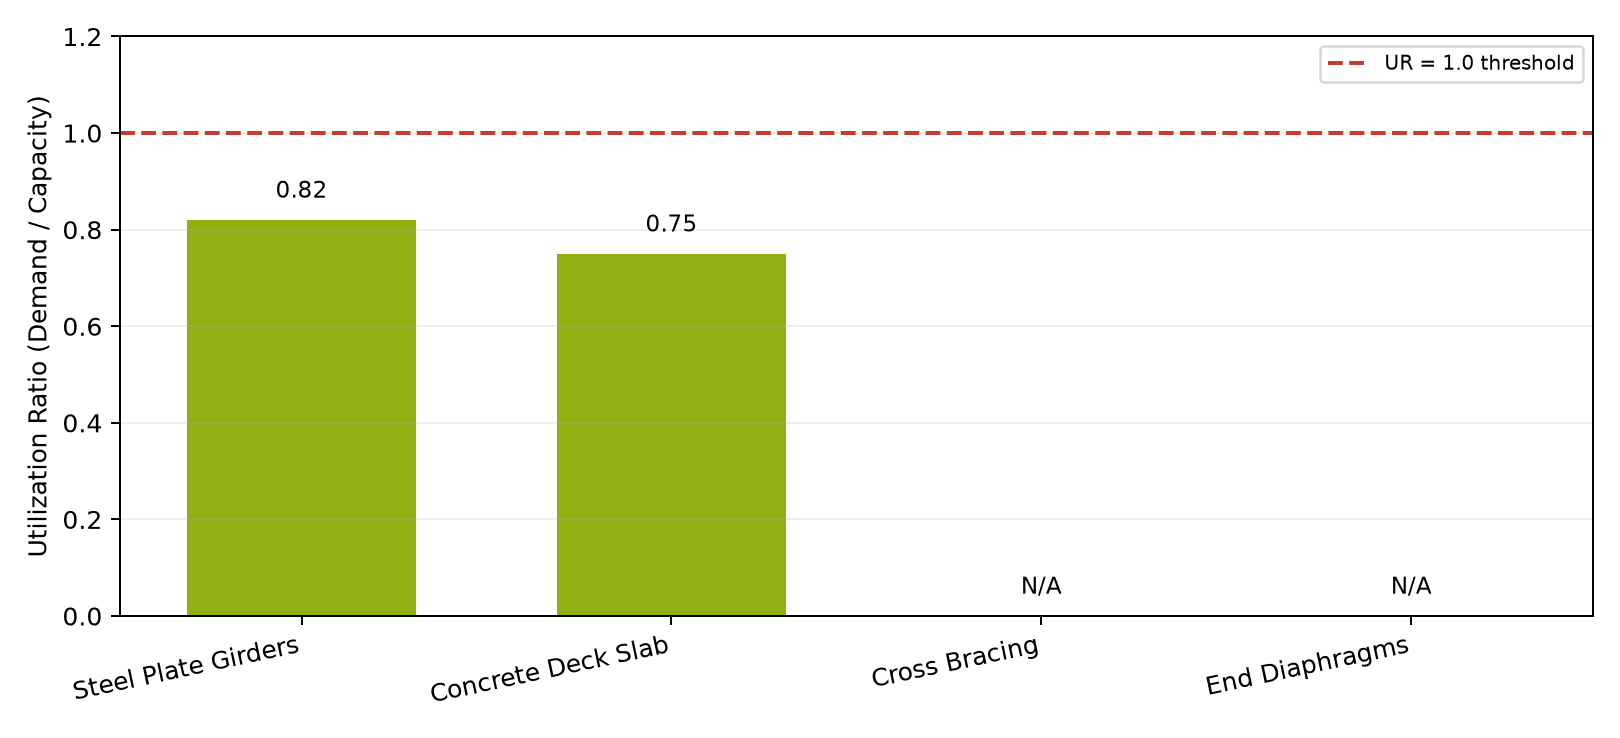
\includegraphics[width=0.88\textwidth]{assets/utilization_summary.png}
\caption{Governing utilization ratio by member family. N/A indicates unavailable design data.}
\end{figure}

\vspace{\reportsectiongap}
\begin{longtable}{|C{3.4cm}|L{4.5cm}|C{2.3cm}|C{2.3cm}|>{\centering\arraybackslash}p{1.6cm}|}
\caption{\textbf{Overall Design Check Summary --- All Members}}\\
\hline
\textbf{Member / Check} & \textbf{Governing Load Combo} & \textbf{Demand} & \textbf{Capacity} & \textbf{UR} \\[\reportrowpad]
\hline
\endfirsthead
\hline
\textbf{Member / Check} & \textbf{Governing Load Combo} & \textbf{Demand} & \textbf{Capacity} & \textbf{UR} \\[\reportrowpad]
\hline
\endhead
Girder --- Moment & --- & 820.00 kNm & 1000.00 kNm & 0.82 \\[\reportrowpad]
\hline
Girder --- Shear & --- & 296.00 kN & 400.00 kN & 0.74 \\[\reportrowpad]
\hline
Girder --- LTB (constr.) & --- & --- & --- & --- \\[\reportrowpad]
\hline
Girder --- Deflection & --- & --- & --- & --- \\[\reportrowpad]
\hline
Girder --- Stress & --- & --- & --- & --- \\[\reportrowpad]
\hline
Girder --- Fatigue & --- & --- & --- & --- \\[\reportrowpad]
\hline
Transverse Shear (slab) & --- & --- & --- & --- \\[\reportrowpad]
\hline
Crack Width (slab) & Frequent SLS & 0.000 mm & 0.000 mm & --- \\[\reportrowpad]
\hline
Deck --- Flexure (sagging) & Basic ULS: 0DL + 0LL & 75.00 kN-m/m & 100.00 kN-m/m & 0.75 \\[\reportrowpad]
\hline
Deck --- Flexure (hogging) & Basic ULS: 0DL + 0LL & 0.00 kN-m/m & 0.00 kN-m/m & --- \\[\reportrowpad]
\hline
Deck --- Cantilever Overhang & Basic ULS: 0DL + 0LL & N/A & N/A & N/A \\[\reportrowpad]
\hline
Deck --- Punching Shear & Basic ULS: 0DL + 0LL & 0.00 MPa & 0.00 MPa & --- \\[\reportrowpad]
\hline
Deck --- One-Way Shear & Basic ULS: 0DL + 0LL & 0.00 kN/m & 0.00 kN/m & --- \\[\reportrowpad]
\hline
Cross Bracing --- Compression & --- & --- & --- & --- \\[\reportrowpad]
\hline
Cross Bracing --- Tension & --- & --- & --- & --- \\[\reportrowpad]
\hline
Cross Bracing --- Slenderness & --- & --- & --- & --- \\[\reportrowpad]
\hline
End Diaphragm --- Moment & \multicolumn{4}{c|}{Rolled / Welded section --- design to be added} \\[\reportrowpad]
\hline
End Diaphragm --- Shear & \multicolumn{4}{c|}{Rolled / Welded section --- design to be added} \\[\reportrowpad]
\hline
\end{longtable}
\noindent\textit{Note: UR = Demand / Capacity. All values $\leq 1.0$ indicate passing checks. The governing check for each component is highlighted in the individual design check sections above.}



\chapter{Drawings and Visualizations}
\label{ch:drawings}

This section presents CAD-generated views of the designed bridge and its components. All views are generated automatically by OsdagBridge using pythonOCC.

\section{Bridge Configuration and Layout}
\label{sec:bridge-layout}

\begin{figure}[H]
\centering
\fbox{\parbox{0.97\textwidth}{
\textit{[ PLACEHOLDER:  Overall 3D Bridge Superstructure ]}
}}
\caption{Overall 3D Bridge Superstructure}
\label{fig:bridge-3d}
\end{figure}


\begin{figure}[H]
\centering
\fbox{\parbox{0.97\textwidth}{
\textit{[ PLACEHOLDER:  Typical Cross Section ]}
}}
\caption{Typical Cross Section}
\label{fig:cross-section}
\end{figure}


\begin{figure}[H]
\centering
\fbox{\parbox{0.97\textwidth}{
\textit{[ PLACEHOLDER:  Top View ]}
}}
\caption{Top View}
\label{fig:top-view}
\end{figure}


\section{Plate Girder --- Detailed Views}
\label{sec:girder-views}

\begin{figure}[H]
\centering
\fbox{\parbox{0.97\textwidth}{
\textit{[ PLACEHOLDER:  3D View of Plate Girders ]}
}}
\caption{3D View of Plate Girders}
\label{fig:girder-3d}
\end{figure}


\begin{figure}[H]
\centering
\fbox{\parbox{0.97\textwidth}{
\textit{[ PLACEHOLDER:  Cross Section of Plate Girder ]}
}}
\caption{Cross Section of Plate Girder}
\label{fig:girder-xsec}
\end{figure}


\begin{figure}[H]
\centering
\fbox{\parbox{0.97\textwidth}{
\textit{[ PLACEHOLDER:  Side View of Girder ]}
}}
\caption{Side View of Girder}
\label{fig:girder-side}
\end{figure}


\section{Cross Bracing Detail}
\label{sec:bracing-detail}

\begin{figure}[H]
\centering
\fbox{\parbox{0.97\textwidth}{
\textit{[ PLACEHOLDER:  Cross Bracing Layout ]}
}}
\caption{Cross Bracing Layout}
\label{fig:cb-layout}
\end{figure}


\noindent
\begin{minipage}[t]{0.31\textwidth}
\centering
\fbox{\parbox{0.95\linewidth}{\centering\textit{[ Cross Bracing -- Bracing Section ]}}}
\captionof{figure}{Cross Bracing -- Bracing Section}
\label{fig:cb-bracing-sec}
\end{minipage}
\hfill
\begin{minipage}[t]{0.31\textwidth}
\centering
\fbox{\parbox{0.95\linewidth}{\centering\textit{[ Cross Bracing -- Top Chord Section ]}}}
\captionof{figure}{Cross Bracing -- Top Chord Section}
\label{fig:cb-top-chord}
\end{minipage}
\hfill
\begin{minipage}[t]{0.31\textwidth}
\centering
\fbox{\parbox{0.95\linewidth}{\centering\textit{[ Cross Bracing -- Bottom Chord Section ]}}}
\captionof{figure}{Cross Bracing -- Bottom Chord Section}
\label{fig:cb-bottom-chord}
\end{minipage}


\section{End Diaphragm Detail}
\label{sec:diaphragm-detail}

\begin{figure}[H]
\centering
\fbox{\parbox{0.97\textwidth}{
\textit{[ PLACEHOLDER:  End Diaphragm Layout ]}
}}
\caption{End Diaphragm Layout}
\label{fig:ed-layout}
\end{figure}


\noindent
\begin{minipage}[t]{0.31\textwidth}
\centering
\fbox{\parbox{0.95\linewidth}{\centering\textit{[ End Diaphragm -- Bracing Section ]}}}
\captionof{figure}{End Diaphragm -- Bracing Section}
\label{fig:ed-bracing-sec}
\end{minipage}
\hfill
\begin{minipage}[t]{0.31\textwidth}
\centering
\fbox{\parbox{0.95\linewidth}{\centering\textit{[ End Diaphragm -- Top Chord Section ]}}}
\captionof{figure}{End Diaphragm -- Top Chord Section}
\label{fig:ed-top-chord}
\end{minipage}
\hfill
\begin{minipage}[t]{0.31\textwidth}
\centering
\fbox{\parbox{0.95\linewidth}{\centering\textit{[ End Diaphragm -- Bottom Chord Section ]}}}
\captionof{figure}{End Diaphragm -- Bottom Chord Section}
\label{fig:ed-bottom-chord}
\end{minipage}



\chapter{Material Take-off \& Quantity Summary}
\label{ch:material-takeoff}

\noindent\textbf{Table 7.1  Bill of Materials (Steel, Concrete, and Reinforcement Quantities)}

\begingroup
\setlength{\tabcolsep}{\reporttabcolsep}
\begin{longtable}{|C{1.0cm}|L{3.8cm}|C{2.6cm}|C{1.8cm}|C{1.8cm}|C{1.8cm}|C{1.8cm}|}
\hline
\textbf{S.N.} & \textbf{Item Description} & \textbf{Volume} & \textbf{Quantity} & \textbf{Total Volume} & \textbf{Weight (MT)} & \textbf{Total Weight (MT)} \\
\hline
\endfirsthead
\hline
\textbf{S.N.} & \textbf{Item Description} & \textbf{Volume} & \textbf{Quantity} & \textbf{Total Volume} & \textbf{Weight (MT)} & \textbf{Total Weight (MT)} \\
\hline
\endhead
1 & Structural Steel (IS 2062) for Girders & N.A. & N.A. & N.A. & N.A. & 42.5 \\
\hline
2(a) & Cross Bracing - Top Chord & N.A. & N.A. & N.A. & N.A. & 1.2 \\
\hline
2(b) & Cross Bracing - Bottom Chord & N.A. & N.A. & N.A. & N.A. & 1.3 \\
\hline
2(c) & Cross Bracing - Diagonal Chord & N.A. & N.A. & N.A. & N.A. & 2.4 \\
\hline
3 & Concrete (M40) for Deck Slab & N.A. & N.A. & 57.6 & N.A. & N.A. \\
\hline
4 & Reinforcement Steel (Fe 500) & N.A. & N.A. & N.A. & N.A. & 6.91 \\
\hline
5 & Shear Stud Connectors & N.A. & N.A. & N.A. & N.A. & N.A. \\
\hline
6 & Crash Barrier & N.A. & N.A. & N.A. & N.A. & N.A. \\
\hline
\end{longtable}
\begin{figure}[H]
\centering
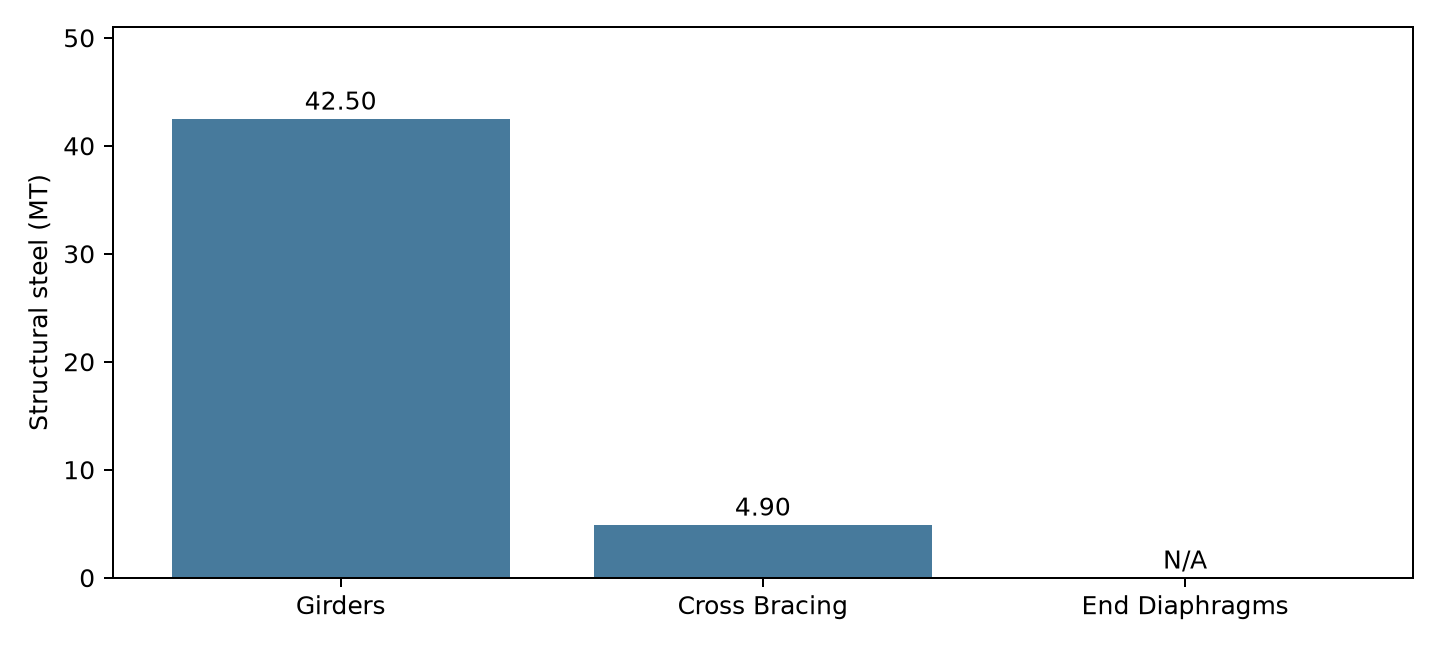
\includegraphics[width=0.88\textwidth]{assets/steel_quantities.png}
\caption{Structural steel quantities by member family (MT).}
\end{figure}

\begin{figure}[H]
\centering
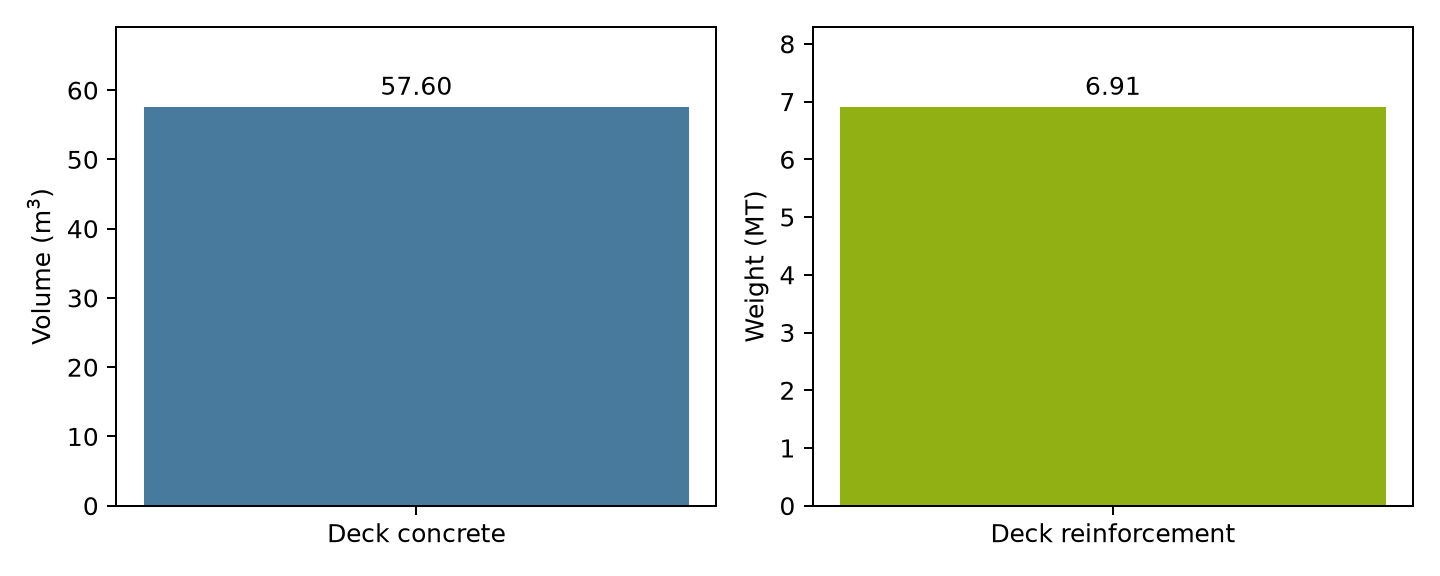
\includegraphics[width=0.88\textwidth]{assets/deck_quantities.png}
\caption{Concrete deck volume and reinforcement steel weight, shown on separate axes.}
\end{figure}


\chapter{Standards \& Assumptions}
\label{ch:Design Standards}

This section provides references to standards used to calibrate the OsdagBridge
design modules, and notes the limitations of the current software version.

\section{Design Standards}
\label{sec:design_standards}

The following Indian Road Congress (IRC) codes and Indian Standards (IS)
form the basis of all design calculations in this software.

\vspace{\reportchaptergap}

\begingroup
\setlength{\tabcolsep}{\reporttabcolsep}
\begin{table}[H]
\caption{\textbf{IRC Codes}}
\begin{tabular}{|c|c|p{13cm}|}
\hline
\textbf{Code} & \textbf{Year} & \textbf{Title / Scope} \\
\hline
IRC 5 & 2015 & General Features of Design - carriageway widths, kerb, footpath dimensions \\
\hline
IRC 6 & 2017 & Loads and Load Combinations - dead load, live load, impact, wind, temperature, etc. \\
\hline
IRC 22 & 2015 & Composite Construction (LS) - Composite section properties, ULS/SLS design, shear connectors \\
\hline
IRC 24 & 2010 & Steel Road Bridges (LS) - Stiffener design, skew angle limits, diaphragm requirements \\
\hline
IRC 112 & 2020 & Concrete Road Bridges - Deck slab flexure, shear, crack width, reinforcement \\
\hline
IRC SP 114 & 2018 & Seismic Design of Road Bridges \\
\hline
\end{tabular}
\end{table}

\begingroup
\setlength{\tabcolsep}{\reporttabcolsep}
\begin{table}[H]
\caption{\textbf{IS Codes}}
\begin{tabular}{|c|c|p{13cm}|}
\hline
\textbf{Code} & \textbf{Year} & \textbf{Scope} \\
\hline
IS 800 & 2007 & Steel construction - tension, compression, bending, shear, LTB, stiffeners, combined checks \\
\hline
IS 456 & 2000 & Concrete - simplified stress-block for deck moment capacity \\
\hline
IS 1786 & 2008 & Reinforcement steel properties \\
\hline
IS 1893 (Part 3) & 2014 & Earthquake resistant design \\
\hline
IS 2062 & 2011 & Structural steel - yield and ultimate strength by grade \\
\hline
\end{tabular}
\end{table}

\clearpage
\section{Analysis and Design Assumptions of This Version}
\label{sec:assumptions}

\textbf{Structural Analysis}

\begin{itemize}
    \item All girders are modelled as simply supported; continuous spans are not currently supported.
    \item A 3D grillage model (OSPGrillage) is used for load distribution. Grillage members carry composite section properties after the construction stage.
    \item The transverse member forces are computed using an approximate 2D frame analogy. For irregular or skewed geometries, a 3D FEM is recommended.
    \item Fixed bearing stiffness is modelled as $k = 1{,}000{,}000 \,\text{kN/m}$ (virtually rigid); free/expansion bearing as $k = 100 \, \text{kN/m}$.
    \item Construction stage sequence analysis is approximate. Detailed staged analysis should be performed for long-term deflection checks.
\end{itemize}

\textbf{Composite Action}

\begin{itemize}
    \item Full shear connection is assumed at ULS with headed stud connectors designed per IRC 22:2015 Cl.606.
    \item Short-term composite section properties (modular ratio $n = E_s/E_{cm}$) are used for ULS checks.
    \item Long-term composite section properties (with creep-adjusted modular ratio) are used for SLS deflection and crack-width checks.
    \item Pre-composite stage: the steel girder alone resists all construction loads prior to concrete gaining strength.
\end{itemize}


\textbf{Material Properties (IRC 22:2015 Annex III)}

\begin{itemize}
\item Steel: $E_s = 200{,}000 \, \text{MPa}, \ G_s = 80{,}000 \, \text{MPa}, \ \nu = 0.30, \ \alpha = 11.7 \times 10^{-6}/^\circ\mathrm{C}$ (grade-independent).
\item Minimum structural concrete grade: M25.
\item Default reinforcement grade: Fe500.
\end{itemize}

\textbf{Partial Safety Factors (IRC 22:2015 Cl.601.4)}

\begin{itemize}
\item $\gamma_{m0}$ (steel yield, ULS) = 1.10
\item $\gamma_{m1}$ (steel ultimate, ULS) = 1.25
\item Reinforcement (ULS) = 1.15
\item Welds -- shop: 1.25; field: 1.50
\item Fatigue ($\gamma_{mft}$) = 1.35
\end{itemize}

\textbf{Loading}

\begin{itemize}
\item Dead load densities per IRC 6:2017 Cl.203: structural steel $78.5 \ \text{kN/m}^3$, concrete $25.0 \ \text{kN/m}^3$, bituminous wearing course $24.0 \ \text{kN/m}^3$.
\item Multi-lane live load reduction factors per IRC 6:2017 Cl.204.4 Table 6A: 1st lane = 1.0, 2nd lane = 0.8, 3rd lane onwards = 0.4.
\item Impact factor (dynamic load allowance) computed from span per IRC 6:2017 Cl.208.2/208.3.
\item Wind load applied as transverse, longitudinal, and vertical components per IRC 6:2017 Cl.209.3.3--209.3.5.
\end{itemize}

\textbf{Serviceability Limits}

\begin{itemize}
\item Deflection limits (IRC 22:2015 Cl.604.3.2): live load + impact $\leq L/800$; total $\leq L/600$.
\item SLS stress limits: concrete $\sigma_c \leq 0.48 f_{ck}$; rebar $\sigma_s \leq 0.80 f_{yk}$; steel $f_e \leq 0.9 f_y$.
\item Permissible crack width: $w_k \leq 0.3 \ \text{mm}$ (bridge deck, exposure class XS2/XD2 per IRC 112:2020 Cl.12.3.2).
\end{itemize}

\textbf{Fatigue}

\begin{itemize}
\item Reference fatigue life: $N_{sc} = 2 \times 10^6$ cycles (IRC 22:2015 Cl.605).
\item Constant stress range is assumed. A thickness correction factor $\mu_r$ is applied for plate thickness $> 25 \ \text{mm}$.
\end{itemize}

\textbf{Stiffener Design}

\begin{itemize}
\item Intermediate transverse stiffener and bearing stiffener design follows IS 800:2007 Cl.8.7.2/8.7.3 and IRC 24:2010 Cl.509.7.2/509.7.3.
\end{itemize}


\section{Known Limitations of This Version}
\label{sec:limitations}

\begin{itemize}
\item Substructure (piers, pile caps, foundations) and bearing design are not included.
\item Splice connection design is not implemented.
\item Skew angle $>$ 15 degrees requires independent manual analysis (IRC 24 Cl. 504.8).
\item Construction stage sequence analysis is approximate; detailed staged analysis
  should be performed for long-term deflection checks.
\item The grillage analysis assumes simply supported boundary conditions;
  continuous spans are not currently supported.
\end{itemize}


\chapter*{References}
\addcontentsline{toc}{chapter}{References}


\begin{enumerate}

\item IRC 5 (2024) --- \textit{Standard Specifications and Code of Practice for Road Bridges, Section I: General Features of Design.}

\item IRC 6 (2017) --- \textit{Standard Specifications and Code of Practice for Road Bridges, Section II: Loads and Load Combinations.}

\item IRC 22 (2014) --- \textit{Standard Specifications and Code of Practice for Road Bridges, Section VI: Composite Construction (Limit State Design).}

\item IRC 24 (2010) --- \textit{Standard Specifications and Code of Practice for Road Bridges, Section V: Steel Road Bridges (Limit State Method).}

\item IRC 112 (2011) --- \textit{Code of Practice for Concrete Road Bridges.}

\item IRC SP 114 (2018) --- \textit{Guidelines for Seismic Design of Road Bridges.}

\item IS 800 (2007) --- \textit{Indian Standard: General Construction in Steel --- Code of Practice.}

\item IS 2062 (2011) --- \textit{Hot Rolled Medium and High Tensile Structural Steel --- Specification.}

\item Subramanian, N. (2008). \textit{Design of Steel Structures.} Oxford University Press.

\item Steel-INSDAG Teaching Resource Materials. \url{https://www.steel-insdag.org}

\end{enumerate}

\end{document}
